%%%%%%%%%%%%%%%%%%%%%%%%%%%%%%%%%%%%%%%%%%%%%%%%%%%%%%%%%%%%%%%%%%%%%%%%%%%%%%%%%%%%%%%%%%%%%%%%%%%%%%%
%%													%%
%% 	BAKALÁŘSKÁ PRÁCE -  Rozšíření zásuvného modulu QGIS pro práci s katastrálními daty
%%                       o podporu veřejně dostupných dat ve formátu VFK			%%
%% 				 Lukáš Kettner						%%
%%													%%
%% pro formátování využita šablona: http://geo3.fsv.cvut.cz/kurzy/mod/resource/view.php?id=775 	%%
%%													%%
%%%%%%%%%%%%%%%%%%%%%%%%%%%%%%%%%%%%%%%%%%%%%%%%%%%%%%%%%%%%%%%%%%%%%%%%%%%%%%%%%%%%%%%%%%%%%%%%%%%%%%% 

\documentclass[%
  12pt,         			% Velikost základního písma je 12 bodů
  a4paper,      			% Formát papíru je A4
  oneside,       			% Oboustranný tisk
  pdftex,				    % překlad bude proveden programem 'pdftex' do PDF
%%%  draft
]{report}       			% Dokument třídy 'zpráva'
%

\newcommand{\Fbox}[1]{\fbox{\strut#1}}

\usepackage[czech, english]{babel}	% použití češtiny, angličtiny
\usepackage[utf8]{inputenc}		% Kódování zdrojových souborů je UTF8

\usepackage[square,sort,comma,numbers]{natbib}

\usepackage{caption}
\usepackage{subcaption}
\captionsetup{font=small}
\usepackage{enumitem} 
\setlist{leftmargin=*} % bez odsazení

\makeatletter
\setlength{\@fptop}{0pt}
\setlength{\@fpbot}{0pt plus 1fil}
\makeatletter

\usepackage[dvips]{graphics}
\usepackage{graphicx}   
\usepackage{color}
\usepackage{transparent}
\usepackage{wrapfig}
\usepackage{float} 

\usepackage{cmap}           
\usepackage[T1]{fontenc}    

\usepackage{textcomp}
\usepackage[compact]{titlesec}
\usepackage{amsmath}
\addtolength{\jot}{1em} 

\usepackage{chngcntr}
\counterwithout{footnote}{chapter}

\usepackage{acronym}
\usepackage{multirow} %pouziti u tabulky, vice radku v jednom
\usepackage[
    unicode,                
    breaklinks=true,        
    hypertexnames=false,
    colorlinks=true, % true for print version
    citecolor=black,
    filecolor=black,
    linkcolor=black,
    urlcolor=black
]{hyperref}         

\usepackage{url}
\usepackage[export]{adjustbox} %pro vycentrovani zadani.jpg
\usepackage{fancyhdr}
%\usepackage{algorithmic}
\usepackage{algorithm}
\usepackage{listings}
\definecolor{backcolour}{rgb}{0.95,0.95,0.92}
\definecolor{codegreen}{rgb}{0,0.6,0}
\lstdefinestyle{mystyle}{
	backgroundcolor=\color{backcolour},
	rulecolor=\color{backcolour},
	captionpos=b,
	numbers=left,
	numbersep=5pt,
	stringstyle=\color{codegreen},
	frame=shadowbox
}
\lstset{style=mystyle}
\usepackage{algcompatible}
\renewcommand{\ALG@name}{Pseudokód}% Update algorithm name
\def\ALG@name{Pseudokód}

\usepackage[
  cvutstyle,          
  bachelor           
]{thesiscvut}


\newif\ifweb
\ifx\ifHtml\undefined % Mimo HTML.
    \webfalse
\else % V HTML.
    \webtrue
\fi 

\renewcommand{\figurename}{Obrázek}
\def\figurename{Obrázek}

%%%%%%%%%%%%%%%%%%%%%%%%%%%%%%%%%%%%%%%%%%%%%%%%%%%%%%%%%%%%%%%%%
%%%%%%%%%%% Definice informací o dokumentu  %%%%%%%%%%%%%%%%%%%%%
%%%%%%%%%%%%%%%%%%%%%%%%%%%%%%%%%%%%%%%%%%%%%%%%%%%%%%%%%%%%%%%%%

%% Název práce
\nazev{Rozšíření zásuvného modulu QGIS pro práci s~katastrálními daty o podporu veřejně dostupných dat ve formátu VFK}{}

%% Jméno a příjmení autora
\autor{Lukáš}{Kettner}

%% Jméno a příjmení vedoucího práce včetně titulů
\garant{Ing.~Martin~Landa,~Ph.D.}

%% Označení programu studia
\programstudia{Geodézie a~kartografie}{}

%% Označení oboru studia
\oborstudia{Geodézie, kartografie a~geoinformatika}{}

%% Označení ústavu
\ustav{Katedra geomatiky}{}

%% Rok obhajoby
\rok{2018}

%Mesic obhajoby
\mesic{únor}

%% Místo obhajoby
\misto{Praha}

%% Abstrakt
\abstrakt{Tato bakalářská práce je zaměřena na rozšíření již
  existujícího softwarového nástroje pro práci s katastrálními daty o
  možnost využití nekomerčních, volně dostupných (nezpoplatněných)
  %% ML: dvakrat v jedne vete: sestaveni a sestavit
  dat ve formátu VFK. Konkrétně se jedná o sestavení bloků PAR a BUD
  (parcel a budov), které lze z dostupných geometrických a popisných
  informací sestavit.  Zásuvný modul bude vyvíjen pro prostředí open
  source nástroje QGIS v programovacím jazyce Python.}  {This bachelor
  %% ML: anglicky text je nutny revidovat, obsahuje preklepy,
  %% stylisticke a gramaticke chyby
  thesis is focused on development of already existing plugin for
  working with cadastral data in VFK format. The project will enable
  the use of non-commercial, for free available data in VFK
  format. That means creat new blocks PAR and BUD (parcels and
  buildings) from geometric and discription information which are
  included. The plugin will be developed in open source project QGIS
  in programming language Python.}

%% Klíčová slova
\klicovaslova
{QGIS, zásuvný~modul, Python, GDAL, VFK}
{QGIS, plugin, Python, GDAL, VFK}

%%%%%%%%%%%%%%%%%%%%%%%%%%%%%%%%%%%%%%%%%%%%%%%%%%%%%%%%%%%%%%%%%%%%%%%%

%%%%%%%%%%%%%%%%%%%%%%%%%%%%%%%%%%%%%%%%%%%%%%%%%%%%%%%%%%%%%%%%%%%%%%%%
%% Nastavení polí ve Vlastnostech dokumentu PDF
%%%%%%%%%%%%%%%%%%%%%%%%%%%%%%%%%%%%%%%%%%%%%%%%%%%%%%%%%%%%%%%%%%%%%%%%
\nastavenipdf
%%%%%%%%%%%%%%%%%%%%%%%%%%%%%%%%%%%%%%%%%%%%%%%%%%%%%%%%%%%%%%%%%%%%%%%

%%% Začátek dokumentu
\begin{document}

\catcode`\-=12  % pro vypnuti aktivniho znaku '-' pouzivaneho napr. v \cline 

% aktivace záhlaví
\zahlavi

% předefinování vzhledu záhlaví
\renewcommand{\chaptermark}[1]{%
	\markboth{\MakeUppercase
	{%
	\thechapter.%
	\ #1}}{}}

% Vysázení přebalu práce
%\vytvorobalku

% Vysázení titulní stránky práce
\vytvortitulku

% Vysázení listu zadani
\stranka{}%
	{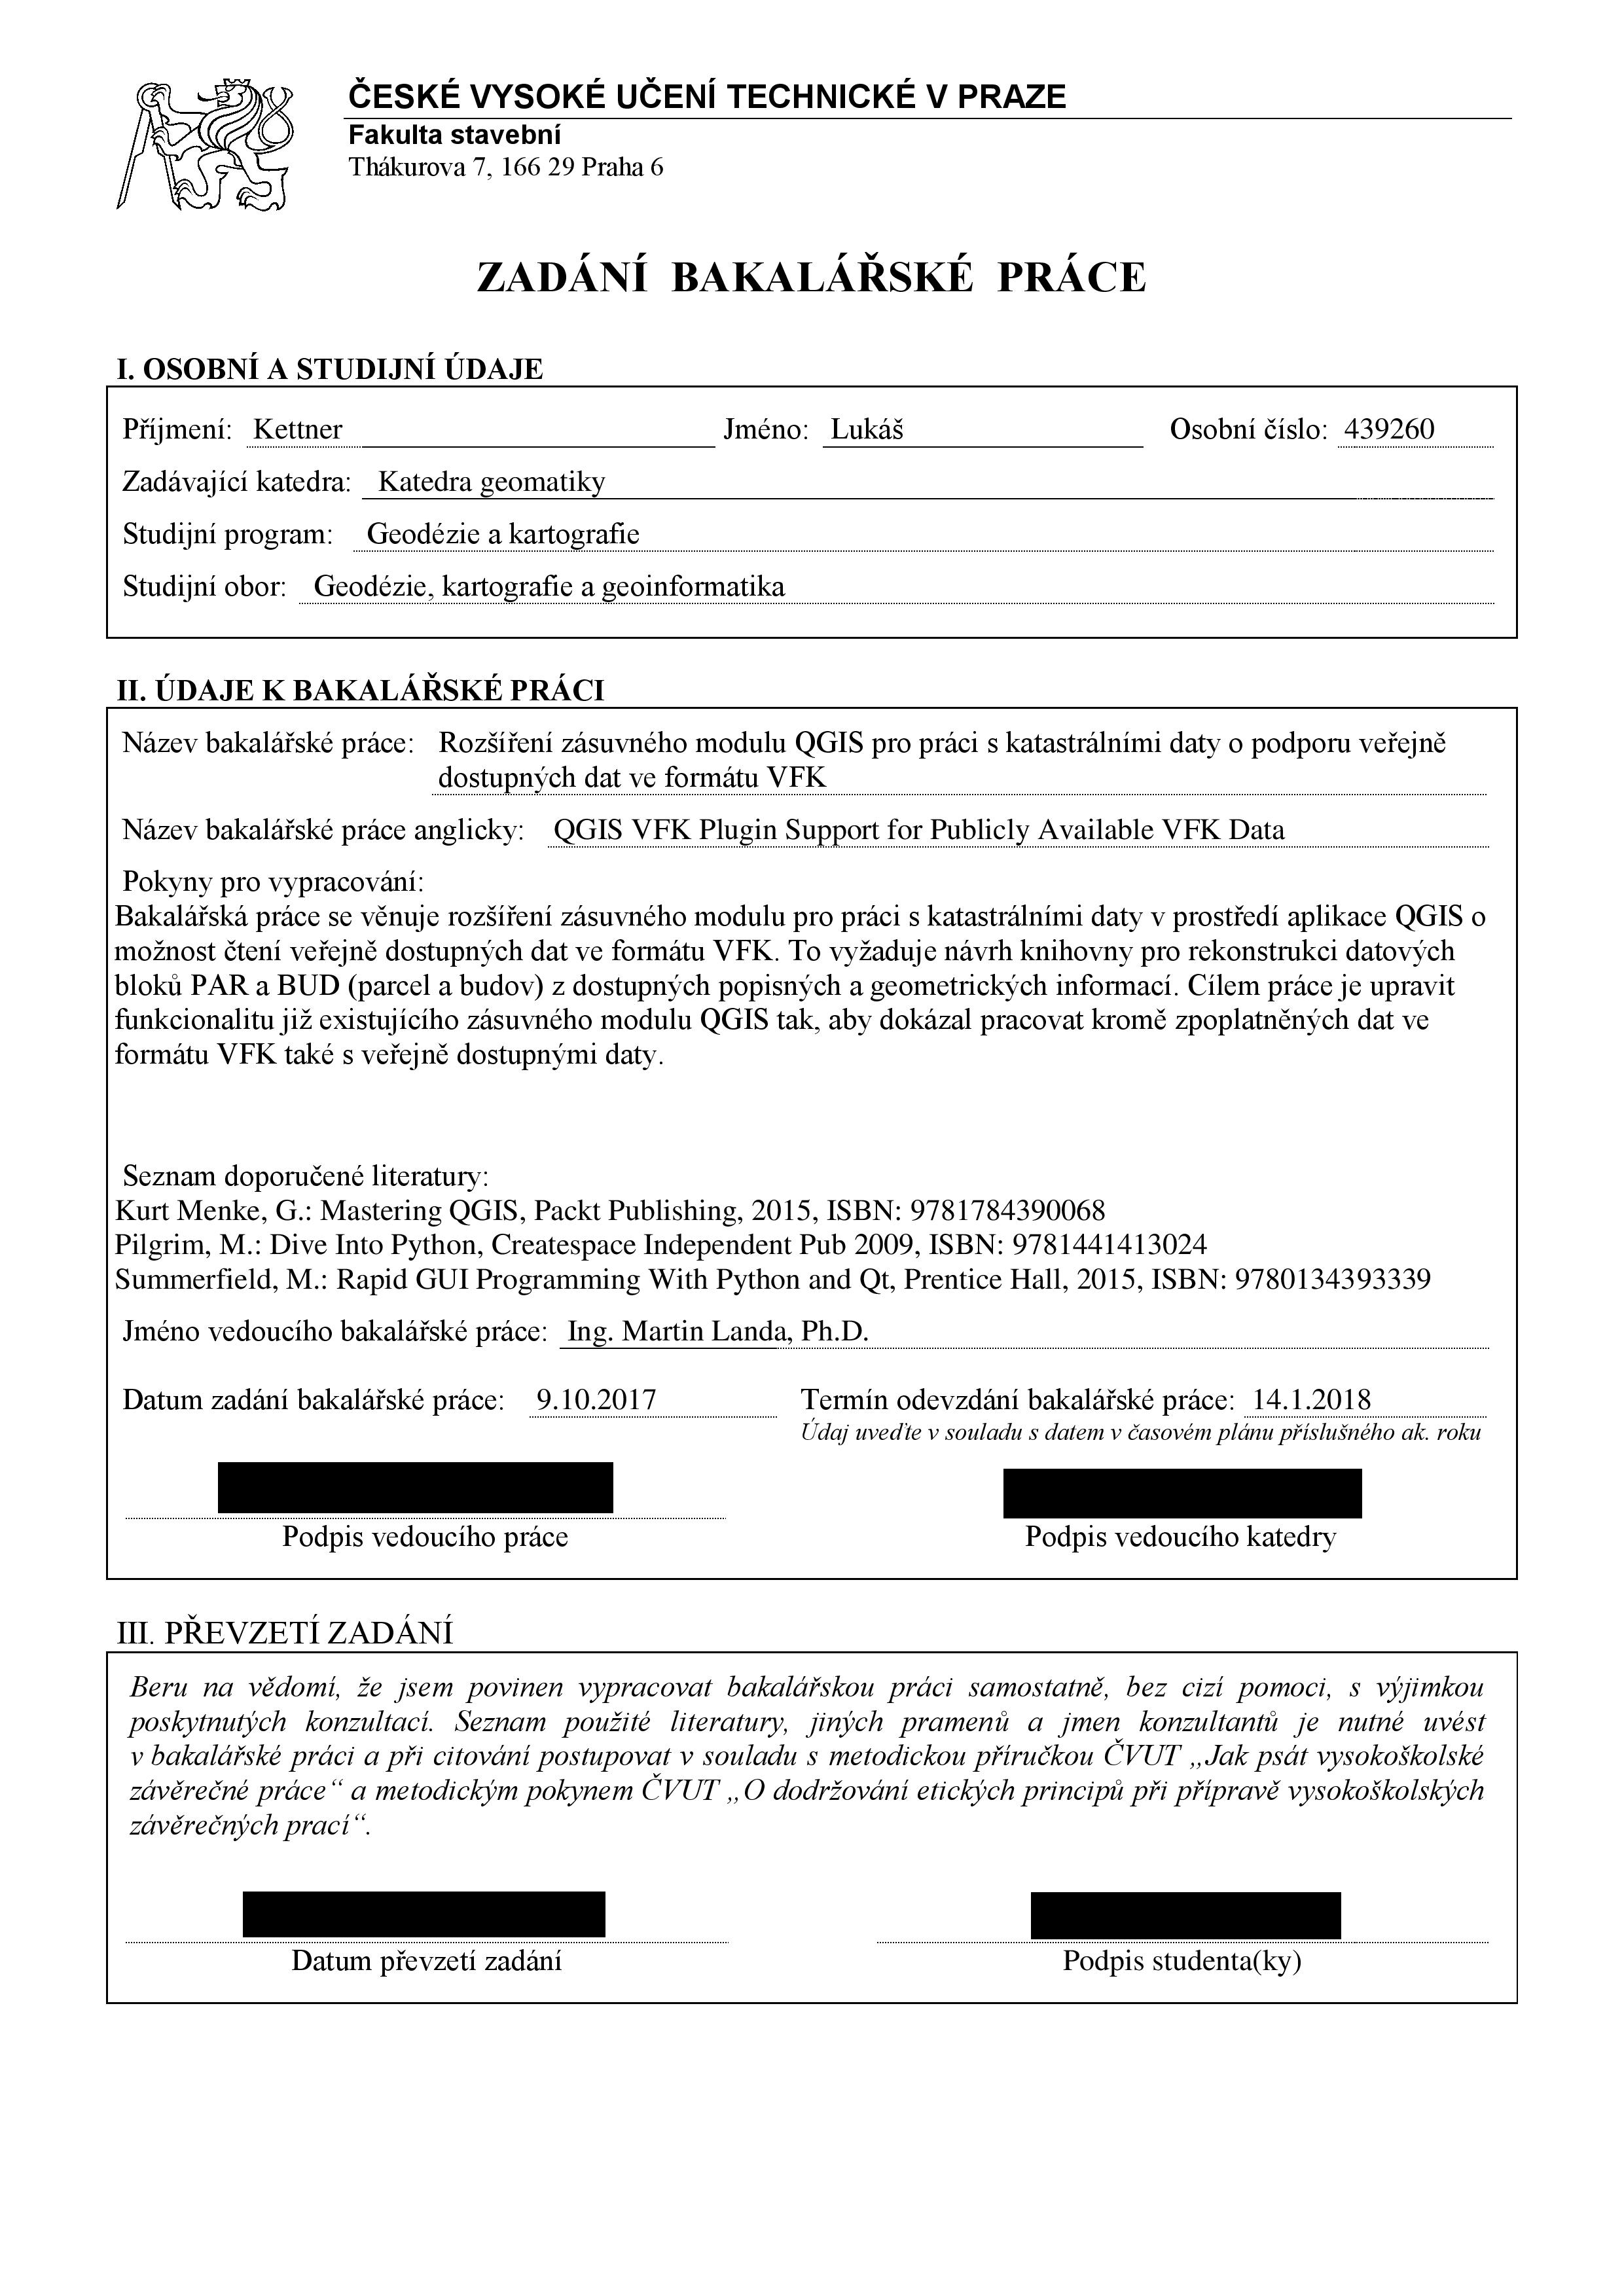
\includegraphics[scale=1, center]{./pictures/zadani.jpg}}%\sffamily\Huge\centering\ }
%ZDE VLOŽIT LIST ZADÁNÍ}%
	%{\sffamily\centering Z~důvodu správného číslování stránek}

% Vysázení stránky s abstraktem
\vytvorabstrakt

% Vysázení prohlaseni o samostatnosti
\vytvorprohlaseni

% Vysázení poděkování
\stranka{%nahore
       }{%uprostred
       }{%dole
       \sffamily
	\begin{flushleft}
		\large
		\MakeUppercase{Poděkování}
	\end{flushleft}
	\vspace{1em}
		%\noindent
	\par\hspace{2ex}
	{Na tomto místě bych chtěl poděkovat především vedoucímu práce, Ing. Martinu Landovi, PhD., nejen za cenné rady a připomínky k zlepšení práce po všech stránkách, ale také za velké množství věnovaného času při objasňování problematiky. Dále chci poděkovat také svým blízkým, kteří mi v případě potřeby byli vždy nápomocni.}
}

% Vysázení obsahu
\obsah

% Vysázení seznamu obrázků
\seznamobrazku

% Vysázení seznamu tabulek
\seznamtabulek

% jednotlivé kapitoly
\chapter{Úvod}
\label{1-uvod}
%Úvod úvodu

%% ML: prvni veta (vybrat poradne) je naprosto nevhodna, jde o
%% vedeckou praci, nejste v hospode ;-), nutne prepsat ML: cely prvni
%% odstavec zni kostrbate, text se Vam rozpada po stylisticke i
%% logicke strance, zkuste cely odstravec prepsat
Téma bakalářské práce jsem si chtěl vybrat pořádně. Zvolit jsem si
chtěl takové téma, které mě zaujme, něco nového se naučím a výsledek
bude ideálně dál využitelný. Proto bylo jasné, že o orientačním běhu,
který je mojí srdeční záležitostí, psát nebudu, poněvadž tím bych moc
nového neobjevil. Výběr tématu jsem začal řešit už v souvislosti s
%% ML: osobni pribeh vynechte, pro volbu tematu nemel az tak zasadni
%% vlic
možným výjezdem do zahraničí, kam jsem chtěl během zimního semestru
vyrazit. To se po návštěvě studijního oddělení ukázalo jako značně
komplikované a proto jsem se rozhodl zůstat s prací na domácí fakultě.

%Proces výběru
Během bakalářského studia mě bavilo programování výpočetních skriptů a
%% ML: na ktery zni kostrbate, zkuste celou vetu prepsat
taky se mi zalíbil geografický informační systém, na který jsme měli
ve třetím ročníku samostatný předmět. Proto jsem s bakalářskou prací
zamířil na katedru geomatiky. První téma, které jsem dostal na
vyzkoušení, byla tvorba zásuvného modulu pro práci s registrem územní
identifikace, adres a nemovitostí. Projekt se jmenoval
\textit{qgis-ruain-plugin} a poprvé jsem si zde vyzkoušel práci s
programovacím jazykem Python. Za úkol jsem měl osahat si prostředí
%% ML: co znamena ``trosku''? Musite byt konkretni a vecny, preci
%% jenom jde o zaverecnou praci technicke povahy, nejde o slohove
%% cviceni
zásuvného modulu a trošku změnit zdrojový kód. Během testování jsem si
samostudiem osvojil základy programovacího jazyka.

%Budoucnost
%% ML: Prvni vetu zkuste prepsat (ubirat svoji)
Práce mě zaujala natolik, že jsem se rozhodl ubírat svojí bakalářskou
práci směrem zásuvného modulu pro geografický informační systém
QGIS. Lákalo mě vyzkoušet si naprogramovat něco užitečného a
funkčního. Zároveň bych si chtěl během tvorby bakalářské práce udělat
%% ML: mozna prilis osobni
jasnější obraz o tom, jakým směrem by se mohla moje studia
ubírat. Stále nemám jasnou volbu mezi geomatikou a inženýrskou
geodézií. Něco mě táhne k geomatice, tak doufám, že mi to bakalářská
práce potvrdí.

%Motivace
%% ML: tady osobni nadech jeste eskaluje, zkuste prepsat ML: uvod
%% pisete v budoucim case, to neni uplne vhodne, text vznika behem
%% prace a nikoliv v minulosti
Začátek nebude jednoduchý, s tím do tvorby práce jdu. Očekávám, že
programování nové knihovny, která je základním kamenem rozšíření
funkcionality zásuvného modulu, bude v hodně věcech podobné psaní
výpočetních skriptů.  Věřím, že zúročím zkušenosti jak z výpočetních
skriptů, tak ze zkušební práce na zásuvném modulu a práce mi půjde
dobře od ruky.

%Představení zadaní
Jako téma práce jsem si zvolil \textit{Rozšíření zásuvného modulu QGIS
  pro práci s katastrálními daty o podporu veřejně dostupných dat ve
  formátu VFK}.  Moje práce bude dál rozšiřovat funkčnost zásuvného
modulu z diplomové práce Bc. Štěpána Bambuly \textit{Rozšíření
  nástroje pro práci s katastrálními daty v programu QGIS}. Práce pana
Bambuly navazovala na již existující nástroj a rozšířila ho o
zpracování a vizualizaci datových vět změnových souborů \zk{VFK}. Dále
nástroj přepsal do jazyka Python, aby usnadnil distribuci zásuvného
modulu v prostředí geografického informačního systému QGIS.

%Cíl práce
%% ML: zvazte prepsani celeho textu do pritomneho casu (Cilem teto
%% prace je...)
Cílem mojí práce bude tento zásuvný modul v jazyce Python ještě
rozšířit o novou knihovnu, která umožní nahrání, prohlížení a
%% ML: spojka 'a' evokuje pocit, ze jde o dve formy, data mohou byt
%% 'neuplna' a take 'verejna': data verejne neobsahuji vsechny datove
%% bloky v porovnani s neverejnymi daty, ktera jsou poskytovana za
%% uplatu
vyhledávání i v neúplných a veřejně dostupných datech ve formátu
\zk{VFK}. Rozšíření bude zaměřené na sestavení bloků PAR a BUD (parcel
a budov), které v těchto datech nejsou obsaženy, ale mohou být z
%% ML: nemluvil bych o 'geometrickych blocich' ale datovych blocich s
%% geometrickou sloznou popisu
přítomných dat sestaveny. Jedná se o dva nejdůležitější geometrické
bloky, které jsou nezbytné pro vizualizaci dat a tvoří datový blok
nemovitostí. Po vytvoření knihovny by měla následovat integrace do již
existujícího zásuvného modulu. Budu se maximálně snažit využít veškeré
v datech obsažené informace, aby se výsledek co nejvíce podobal datům
úplným. Tím dojde i k zachování většiny funkcí rozšiřovaného zásuvného
modulu.

%Struktura práce
%% ML: po presani do pritomneho casu, muzete pridat odkazy na
%% jednotlive kapitoly
Samotná práce bude logicky uspořádána do dvou celků. Prvním bude
teoretická část zabývající se představením informačního systému
katastru nemovitostí(\zk{ISKN}) a jeho historie. Dále bude rozebrána
základní struktura výměnného formátu katastru (\zk{VFK}), ve kterém
jsou data poskytována. Přidám porovnání úplného a neúplného formátu
doplněné o přehled datových bloků, pro které je nutné sestavit
geometrii, aby šlo bloky PAR a BUD knihovnou také sestavit. Představím
použitou technologii, kam patří například programovací jazyk Python a
knihovnu GDAL.

Druhá část už bude zaměřená čistě na praktickou stránku
práce. Podrobně představím funkcionalitu jednotlivých tříd a členských
metod z nově vzniklé knihovny a také funkčnost knihovny
samotné. Součástí praktické části bude i integrace vzniklé knihovny do
již existujícího zásuvného modulu, která bude také představena a
doplněna o ukázky načítání dat.

%%%POZNAMKY
%-Data výměnného formátu katastru(\zk{VFK}) jsou poskytována ve dvou podobách.

%Rešerše% \textbf{Rešerše:} 
%Odkaz v textu% \footnote{\url{http://theses.cz/id/o3vhp8/Diplomov_prce_Lokov.pdf}}
%Kurzíva% \textit{}
%Zkratka% \zk{ZHN}
%\footnote{}

\chapter{Teoretický základ}
\label{2-teorie}
%co v kapitole uvedu?
V této kapitole bude představen Informační systém katastru nemovitostí, způsob poskytování dat z katastru nemovitostí a výměnný formát katastru nemovitostí včetně struktury formátu. Text této kapitoly vychází z informací o \zk{ISKN} na webové stránce \zk{ČUZK},viz \cite{iskn}.

\section{Informační systém katastru nemovitostí}
Katastr nemovitostí se řadí mezi datově nejrozsáhlejší informační systémy státní správy. Pro výkon státní správy a zajištění uživatelských služeb byl v letech 1997-2001 zřízen Informační systém katastru nemovitostí(\zk{ISKN}), který sjednotil vedení a správu katastru nemovitostí do jediného informačního systému. Aktuální data z katastru nemovitostí jsou dostupná přes službu Dálkový přístup na síti internet po registraci během několika minut. 
%zdroj: http://www.cuzk.cz/Katastr-nemovitosti/O-katastru-nemovitosti/Informacni-system-katastru-nemovitosti-ISKN.aspx
\subsection{Vývoj ISKN}
\zk{ISKN} vznikl v letech 1997 -- 2001 ve spolupráci s firmou APP Czech s.r.o.(NESS Czech s.r.o.). V roce 1998 došlo k dokončení digitalizace souboru popisných informací a nyní se digitalizuje souboj geodetických informací. Na všech katastrálních pracovištích byl \zk{ISKN} zprovozněn v roce 2001. Během následujících let byl systém průběžně laděn. V letech 2007 až 2010 došlo k centralizaci informačního systému do jediné databáze, čímž odpadlo replikování ze 107 lokálních databází a zrychlila se aktualizace dat ve webové aplikaci Dálkový přístup. Velkou výhodou \zk{ISKN} je možnost zavedení automatických kontrol při zápisu do katastru nemovitostí. Kvůli zvýšení bezpečnosti, na kterou byl při tvorbě systému kladen velký důraz, je celá infrastruktura zdvojena. Vzniklo tak primární a záložní centrum, které v případě výpadku primárního centra udrží \zk{ISKN} v provozu.
\subsection{Poskytování dat}
Český úřad zeměměřický a katastrální(\zk{ČUZK}) poskytuje široké spektrum data v digitální podobě. Data je možné stahovat přes službu Dálkový přístup k údajům katastru nemovitostí České republiky, která je zpoplatněná a přístupná registrovaným uživatelům na adrese:~\href{https://www.cuzk.cz/aplikace-dp}{https://www.cuzk.cz/aplikace-dp}. Nebo přes Služby mapového serveru na adrese:~\href{http://services.cuzk.cz/}{http://services.cuzk.cz}, kde jsou služby poskytovány bezúplatně.

Zpoplatněná data ve výměnném formátu \zk{ISKN} v textovém tvaru, poskytovaná přes webovou aplikaci Dálkový přístup, obsahují popisné i grafické informace dle zadané kombinace bloků(viz.~\ref{tab:komb_dat_skup}).

Práce bude zaměřená na využití bezúplatně poskytnutých dat katastrální mapy z Neharmonizované služby. Katastrální mapa je ke stažení ve formátech \zk{VFK}(aktualizace měsíčně), SHP\footnote{Shapefile je formát pro ukládání prostorových dat}(aktualizace týdně) a DGN\footnote{Grafický formát dat určený pro "kreslící" softwary}(aktualizace denně). 

 %http://www.gisoft.cz/Moduly/ImportVFK
\begin{table}[h!] %specifikace umisteni objektu-tabulky, ! trvá na umístění h-here
			\centering
			\caption{Kombinace datových bloků(zdroj:
\href{http://www.cuzk.cz/Katastr-nemovitosti/Poskytovani-udaju-z-KN/Vymenny-format-KN/Vymenny-format-NVF.aspx}{cuzk.cz})}
			\label{tab:komb_dat_skup}
			\begin{tabular}{|l|l|}
				\hline
				\textbf{Blok}           	& \textbf{Popis bloku}  	\\ \hline
				1. Nemovitosti				& parcely a budovy	\\ \hline
				2. Jednotky					& bytové jednotky	 \\ \hline
				3. Bonitní díly parcel      & kódy \zk{BPEJ} k parcelám              \\ \hline
				4. Vlastnictví             	& listy vlastnictví, oprávněné subjekty a vlastnické vztahy		 \\ \hline
				5. Jiné právní vztahy 		& ostatní právní vztahy kromě vlastnictví \\ \hline
				6. Řízení       			& údaje o řízení (vklad, záznam,…) a listiny          \\ \hline
				7. Prvky katastrální mapy 	& katastrální mapy v digitální podobě	 \\ \hline
				8. \zk{BPEJ}				& hranice \zk{BPEJ} včetně kódů	 \\ \hline
				9. Geometrický plán			& geometrické plány	 \\ \hline
				10. Rezervovaná čísla		& rezervovaná parcelní čísla a čísla \zk{PBPP}	 \\ \hline
				11. Definiční body 			& definiční body parcel a staveb	 \\ \hline
				12. Adresní místa 			& adresní místa budov	 \\ \hline
			\end{tabular}
		\end{table}
%tabulka zdroj: http://www.cuzk.cz/Katastr-nemovitosti/Poskytovani-udaju-z-KN/Vymenny-format-KN/Vymenny-format-NVF.aspx
Poskytování veškerých dat se řídí vyhláškou číslo 358/2013 Sb., o poskytování údajů z katastru nemovitostí.
\section{Výměnný formát katastru nemovitostí}
Obsah této kapitoly vychází z informací na stránkách \zk{ČUZK} o Výměnném formátu katastru nemovitostí a z oficiálního dokumentu o výměnném formátu katastru \textit{Struktura výměnného formátu informačního systému katastru nemovitostí České republiky} ze dne 7.11.2014 \cite{struktura_ISKN}.
\subsection{Historie a vývoj}
Výměnný formát před vznikem \zk{ISKN} byl označován jako \textit{starý výměnný formát(SVF)} a obsahoval tři samostatné a oddělené části:
\begin{itemize}[leftmargin=50pt]
	\item \textbf{Soubor popisných informací(SPI)} - informace o parcelách, vlastnících, nabývacích titulech
	\item \textbf{Soubor geodetických informací (SGI)} - informace o poloze nemovitosti
	\item \textbf{Digitální katastrální mapu (DKM)} - soubory ve formátu VKM
\end{itemize}
%zdroj: http://www.cuzk.cz/Katastr-nemovitosti/Poskytovani-udaju-z-KN/Vymenny-format-KN/Vymenny-format-KN-pred-ISKN.aspx
Podpora starého výměnného formátu skončila se vznikem \zk{ISKN}, protože v něm jsou data popisná a geodetická uložena ve společném datovém modulu. Proto byl vytvořen a postupně implementován \textit{nový výměnný formát(NVF)}. Jeho data jsou poskytována ve dvou časových režimech:

\begin{itemize}[leftmargin=50pt]
\item \textbf{Prvotní data} -- kompletní data pro konkrétní časové období						
\item \textbf{Změny} -- data obsahující pouze změny za konkrétní časové období, lze zadávat datum od-do včetně času					 
\end{itemize}
Tento nový datový formát obsahuje dle požadované kombinace bloků popisnou i grafickou informaci včetně dat o řízení. Rozsah poskytovaných dat je možné definovat podle:

\begin{itemize}[leftmargin=50pt]
		\item Územní jednotky (katastrální území, obec, okres, Česká republika)
		\item Oprávněného subjektu
		\item Výběrem parcel
		\item Výběrem parcel polygonem v mapě
\end{itemize}
%http://www.cuzk.cz/Katastr-nemovitosti/Poskytovani-udaju-z-KN/Vymenny-format-KN/Vymenny-format-ISKN-v-textovem-tvaru.aspx
%http://geo.fsv.cvut.cz/~landa/publications/2005/diploma_thesis/martin.landa-thesis.pdf
\subsection{Struktura výměnného formátu ISKN}
V této kapitole bude představena základní struktura nového výměnného formátu \zk{ISKN}. Detailní popis je k dispozici v oficiální dokumentaci o struktuře\cite{struktura_ISKN}.

Výměnný formát je určený k vzájemnému předávání dat mezi systémem \zk{ISKN} a jinými systémy zpracování dat. Datový soubor výměnného formátu je textový soubor s kódováním češtiny\footnote{Pouze ve výjimečných případech lze poskytnout v kódování dle WIN1250} dle ČSN ISO 8859-2 (ISO Latin2) skládající se z:
\begin{itemize}[leftmargin=50pt]
		\item hlavičky \verb|&H|
		\item datových bloků \verb|&B|
		\item koncového znaku \verb|&K|
\end{itemize}
Každý z datových bloků v sobě obsahuje informaci o atributech a jejich formátu následovanou vlastními datovými řádky. Každá věta hlavičky (\verb|&H|), definice bloku(\verb|&B|) i věta dat (\verb|&D|) je zakončena znaky <CR><LF> pro konec řádku a začátek nového. %ukázku?

Hlavička textového souboru výměnného formátu katastru obsahuje podrobné informace o:
\begin{itemize}[leftmargin=50pt]
		\item verzi dat
		\item datu a času vytvoření
		\item původu dat
		\item označení kódové stránky
		\item obsažených datových blocích
		\item osobě, která soubor vytvořila
		\item časové podmínce použité pro vytvoření souboru
		\item omezujících podmínkách (katastrální území, oprávněné subjekty, parcely, polygon)
\end{itemize}
V ukázce hlavičky~\ref{lst:hlavicka} jsou podrobné informace o textovém souboru zřejmé. Pořadí řádků ukázky hlavičky odpovídá předchozímu vypsanému pořadí jednotlivých informací.
\begin{lstlisting}[caption=Ukázka hlavičky neúplných dat, label=lst:hlavicka]
&HVERZE;"5.1"
&HVYTVORENO;"03.03.2017 14:37:03"
&HPUVOD;"ISKN"
&HCODEPAGE;"WE8ISO8859P2"
&HSKUPINA;"PKMP";"BPEJ"
&HJMENO;"system"
&HPLATNOST;"01.03.2017 00:00:00";"01.03.2017 00:00:00"
&HZMENY;0
&HNAVRHY;0
&HPOLYG;0
\end{lstlisting}

Po hlavičce následuje v textovém souboru \zk{VFK} datový blok výměnného formátu \zk{ISKN}. Datový blok počíná uvozovacím řádkem, který se skládá ze znaku \verb|&B|(blok výměnného formátu) a zkratky příslušného bloku. Dále je v uvozovacím řádku seznam atributů včetně datového formátu. Datový formát N je číselný, T textový a D datumový. Číslice za datovým formátem uvádí maximální délku položky u všech formátů. U číselného formátu může být definován počet číslic před a za desetinnou čárkou pomocí dvou číslic oddělených tečkou. Jednotlivé atributy jsou odděleny středníkem, viz ukázka~\ref{lst:datovy_blok}.

{\small
\begin{lstlisting}[caption=Ukázka datového bloku SOBR(souřadnice obrazu bodů polohopisu v mapě) neúplných dat, label=lst:datovy_blok]
&BSOBR;ID N30;STAV_DAT N2;KATUZE_KOD N6;CISLO_ZPMZ N5;
CISLO_TL N4;CISLO_BODU N12;UPLNE_CISLO N12;SOURADNICE_Y N10.2;
SOURADNICE_X N10.2;KODCHB_KOD N2
&DSOBR;2187300403;0;600016;346;;5;3460005;851356.47;995318.95;
&DSOBR;2187306403;0;600016;346;;25;3460025;851364.89;995306.02;
&DSOBR;2219969403;0;600016;367;;9;3670009;850092.23;996905.77;
\end{lstlisting}}

\subsection{Struktura neúplných data výměnného formátu katastru}
\label{subsec:neuplna_data}
Úplná data výměnného formátu katastru nemovitostí, která jsou zpoplatněna a poskytována přes webovou aplikaci Dálkový přístup, obsahují následujících 12 skupin datových bloků: \verb|&HSKUPINA;"NEMO"|; \verb|"JEDN";"BDPA"|; \verb|"VLST";"JPVZ"|; \verb|"RIZE";"PKMP"|; \verb|"BPEJ";"GMPL"|; \verb|"REZE";"DEBO";"ADRM"|, viz tabulka~\ref{tab:komb_dat_skup}.

Data neúplná obsahují pouze dvě skupiny datových bloků, jak je vidět v ukázce hlavičky neúplných dat~\ref{lst:hlavicka}--řádek 5. Kvůli nepřítomnosti dalších datových skupin jsou data označována jako neúplná. Obsaženy jsou skupiny bloků PKMP a BPEJ, které vlastně tvoří kompletním katastrální mapu. Popisné informace data neobsahují.

\begin{table}[h!] %specifikace umisteni objektu-tabulky, ! trvá na umístění h-here
\begin{center}
			%\centering
			\caption{Skupiny datových bloků v neúplných datech \zk{VFK}(zdroj:\cite{struktura_ISKN})}
			\label{tab:Seznam skupin datových bloků neúplného výměnného formátu ISKN}
			\scalebox{0.75}{
			\begin{tabular}{|c|l|l|l|l|}
			\hline
			\multicolumn{2}{|c|}{Skupina} & \multicolumn{2}{|c|}{Datový blok}\\ \hline
			{Jméno}          & {Kód}  & {Kód}  	&{Popis}\\ \hline
			\multirow{15}{6em}{Prvky katastrální mapy}	& \multirow{15}{*}{PKMP} 	&SOBR 	&Souřadnice obrazu bodů polohopisu v mapě\\ \cline{3-4}
			&  &SBP					&Spojení bodů polohopisu -- definuje polohopisné liniové prvky\\ \cline{3-4}
			&  &SBM					&Spojení bodů mapy -- definuje nepolohopisné liniové prvky \\ \cline{3-4}
			&  &KODCHB				&Číselník kódů charakteristiky kvality bodu \\ \cline{3-4}
			&  &TYPSOS				&Číselník typů souřadnicových systémů \\ \cline{3-4}
			&  &HP(PL)				&Hranice parcel\\ \cline{3-4}
			&  &OP(NL, NB)			&Obrazy parcel (parcelní číslo, značka druhu pozemku, ...) \\ \cline{3-4}
			&  &OB(PL, NB)			&Obrazy budov (obvod budovy, značka druhu budovy)\\ \cline{3-4}
			&  &DPM(NB, PB, NL, PL)&Další prvky mapy\\ \cline{3-4}
			&  &OBBP(PB, NB)		&Obrazy bodů BP\\ \cline{3-4}
			&  &TYPPPD				&Číselník typů prvků prostorových dat\\ \cline{3-4}
			&  &ZVB					&Zobrazení věcných břemen\\ \cline{3-4}
			&  &POM					&Prvky orientační mapy\\ \cline{3-4}
			&  &SPOM				&Spojení prvků orientační mapy -- definuje liniové prvky\\ \cline{3-4}
			&  &SPOL				&Souřadnice polohy bodů polohopisu (měřené)\\ \hline
				\multirow{2}{*}{BPEJ}	& \multirow{2}{*}{BPEJ}			&HBPEJ(NL)			&Hranice BPEJ\\ \cline{3-4}
										& 								&OBPEJ(NB)			&Označení BPEJ\\ \hline
			\end{tabular}}
			\end{center}
		\end{table}
Zkratky u kódu datového bloku nesou upřesňující informaci o geometrii bloku: NB -- nepolohopisný bodový prvek, PB -- polohopisný bodový prvek, NL -- nepolohopisný liniový prvek, PL -- polohopisný liniový prvek.
		
Skupina Prvky katastrální mapy obsahuje celkem 15 datových bloků, které tvoří katastrální mapu. Skupina datových bloků \zk{BPEJ} obsahuje hranice a označení bonitované půdně ekologické jednotky, která je základní mapovací a oceňovací jednotkou zemědělské půdy.
\subsection{Stažení neúplných dat výměnného formátu katastru}
Tato bakalářská práce je zaměřená na zpracování bezúplatně poskytovaných data z neharmonizovaných služeb mapového serveru \zk{ČUZK}, kde jsou všechny služby poskytovány bezúplatně. Data je možné stáhnout z internetu na adrese \href{http://services.cuzk.cz/vfk/}{http://services.cuzk.cz/vfk/}, kde je zvoleno jestli jsou požadovány soubory s katastrální mapou po katastrálním území(označeno \textit{ku}) nebo katastrálním pracovišti(označeno \textit{kp}). Poté se zvolí z jakého měsíce mají data být, vždy vztaženo k prvnímu dni v měsíci. Ke stažení jsou data aktuální případně až tři měsíce stará. V posledním okně se volí konkrétní katastrální území nebo pracoviště podle názvu.
%http://freegis.fsv.cvut.cz/gwiki/V%C3%BDm%C4%9Bnn%C3%BD_form%C3%A1t_ISKN
\subsection{Bloky parcel a budov}
\label{subsec:bloky_par_bud}
Oba datové bloky patří do skupiny datových bloků s názvem Nemovitosti a kódem NEMO a jsou obsaženy pouze v úplných datech.

Datový blok PARCELY s kódem PAR obsahuje parcely evidované v \zk{ISKN}. S využitím sloupců \verb|PAR_ID_1| a \verb|PAR_ID_2| z datového bloku HP (hranice parcel) je možné získat seznam okolních parcel dané parcely. Blok BUDOVY s kódem BUD obsahuje stavby evidované v \zk{ISKN}.
 
\section{Nástroje pro čtení dat VFK} 
Na čtení dat Informačního systému katastru(\zk{ISKN}) je k dispozici poměrně velké množství prostředků. Některé jsou komerční a jiné volně dostupné. V následující kapitole budou představeny dohledané softwary včetně v praxi využitého VFK driveru(\ref{subsec:gdal_vfk}). Pokud to bylo možné, načtení dat bylo v jednotlivých softwarech ozkoušeno.
\subsection{GISOFT}
Jedná se o komerční modul od společnosti GISoft ve spolupráci se společností Bentley Systems pro MicroStation. Modul umožňuje import dat v novém i starém výměnném formátu katastru nemovitostí České republiky. Tento modul je k dispozici pro nadstaveby MGEO a SPIDER.\cite{gisoft}

\begin{figure}[H]
	 \centering
      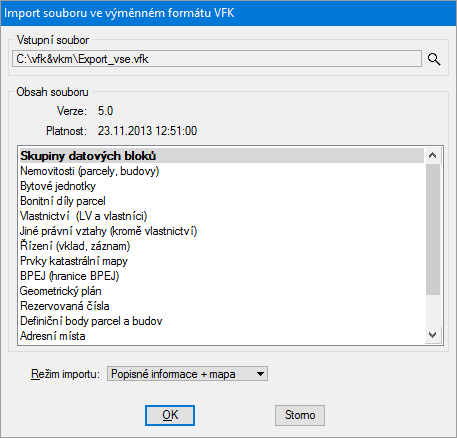
\includegraphics[height=9cm]{./pictures/gisoft.png}
      \caption{Ukázka načtení VFK dat (zdroj:
\href{http://www.gisoft.cz/cze/files/Moduly/import-vfk.png}{gisoft.cz})}
      \label{fig:gisoft}
  \end{figure}
%zdroj: http://www.gisoft.cz/Moduly/ImportVFK
%obrazek: http://www.gisoft.cz/cze/files/Moduly/import-vfk.png
\subsection{Spirit VFK}
Samospustitelná desktopová aplikace určená pro převod dat katastru nemovitostí do libovolné geodatabáze ESRI. Do geodatabáze jsou importovány tabulky, relace a ostatní databázové objekty \zk{ISKN}. Výslednou databázi lze použít pro analytickou práci na datech kastartu nemovitostí nebo v aplikačních nadstavbách \textit{Spirit KN} a \textit{Spirit Portál}-KN. Produkt je od společnosti GEOREAL s.r.o. a je zpoplatněný. Po krátké registraci je možné vyzkoušet 30-ti denní Trial verzi \footnote{http://mapy.georeal.cz/trialreg/}.\cite{spirit_vfk}
%zdroj: http://www.georeal.cz/cz/spirit-desktop/spirit-vfk
\subsection{TopoL xT}
TopoL xT je zpoplatněný software od společnosti TopoL. Je to obecný geografický systém určený pro přípravu, správu a analýzu geografických dat. Soubory výměnného formátu katastru nemovitostí(\zk{VFK}) jsou jedním z podporovaných formátu při importu. Pro vyzkoušení je k dispozici demonstrační verze\footnote{http://www.topol.eu/files/download/topol/100/setup.exe}, ve které je omezený počet objektů, omezená velikost rastru a nelze tisknout v měřítku.\citep{topol}

\begin{figure}[H]
	 \centering
      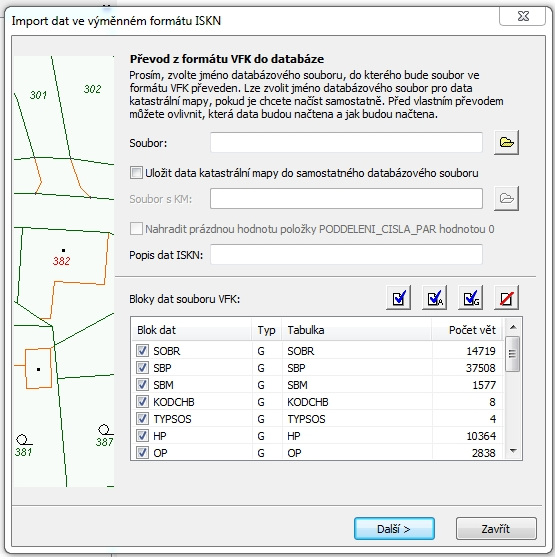
\includegraphics[height=9cm]{./pictures/topol.png}
      \caption{Ukázka importu VFK dat v programu TopoL xT (zdroj:vlastní)}
      \label{fig:topol}
  \end{figure}
%http://www.topol.eu/articles/software#topol-xt
\subsection{Kokeš}
Interakční grafický systém Kokeš od firmy GEPRO s.r.o. je zaměřený na obor geodézie a na geoinformační systémy. V systému je možné řešit nejrůznější geodetické i konstrukční výpočty, vytvářet a aktualizovat kresby map, vést popisné údaje k objektům a bodům mapy, digitalizovat grafické podklady. Budování systému po základních a uživatelských funkcích umožňuje postupný vývoj a jednoduché ovládání. \cite{kokes_cvut}

Funkce import \zk{VFK} umožňuje importovat jednotlivé soubory, kdy vstupem je jeden nebo více souborů \zk{VFK} (nebo ZIP) a výsledkem je jedna databáze SPI a výkresy katastrální mapy, orientační mapy, definičních bodů parcel a definičních bodů budov. %\citep{napoveda_kokes}

\begin{figure}[H]
	 \centering
      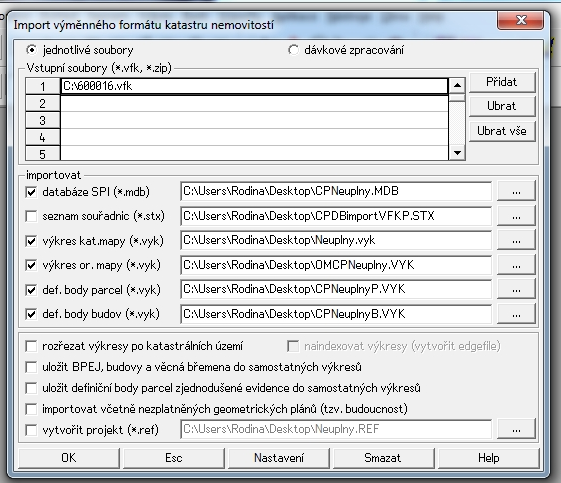
\includegraphics[width=10cm]{./pictures/kokes.png}
      \caption{Ukázka importu VFK dat v programu Kokeš (zdroj:vlastní)}
      \label{fig:kokes}
  \end{figure}
  
Informace o Funkci import \zk{VFK} pocházejí z nápovědy k funkci dostupné v samotném programu.
%zdroj: http://geo3.fsv.cvut.cz/~soukup/dip/bukovsky/1.htm, napoveda kokes k funkci import vfk
\subsection{ISKN Studio pro ArcGIS}
Software určený pro import dat formátu \zk{ISKN} do formátu geodatabáze. Pracuje s daty ve formátu NVF a umožňuje jejich zpracování do osobní, souborové a ArcSDE geodatabáze v MS SQL Server či Oracle. K ISKN Studiu je možné doinstalovat doplněk ISKN View, který slouží k rychlému a jednoduchému vyhledávání v datech ISKN převedených pomocí softwaru ISKN Studio. Jedná se o zpoplatněný software. \cite{arcgis}

\begin{figure}[H]
	 \centering
      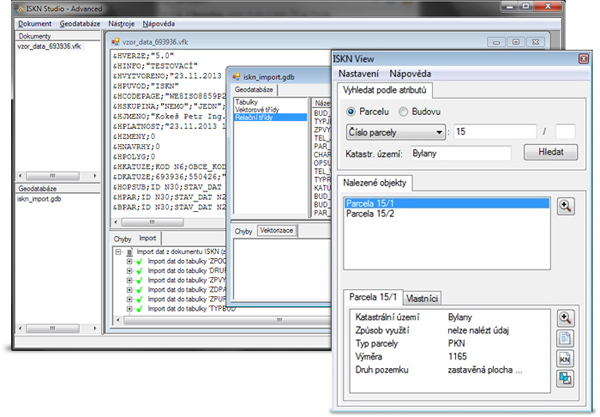
\includegraphics[height=9cm]{./pictures/iskn_studio.jpeg}
      \caption{Ukázka načtení VFK dat v ISKN Studiu (zdroj:
\href{https://www.arcdata.cz/uploads/media/general/0001/01/68f0bfd90cf19d903a57fc8457e1f228a7dd47f4.jpeg}{arcdata.cz})}
      \label{fig:ISKNStudio}
  \end{figure}
%zdroj:https://www.arcdata.cz/produkty/software-arcdata/import-iskn
%obrázek: https://www.arcdata.cz/uploads/media/general/0001/01/68f0bfd90cf19d903a57fc8457e1f228a7dd47f4.jpeg
\subsection{cadstudio}
V obou případech se jedná o konverzní aplikaci firmy CAD Studio určenou pro zpracování dat \zk{ISKN}.
\begin{itemize}[leftmargin=50pt]
\item VFK2DB -- import dat do relační databáze Oracle nebo MS SQL Server, samostatně spustitelný program \cite{vfk2db} %http://www.cadstudio.cz/vfk
\item VFK2DWG -- automatický převod souboru či souborů VFK přímo na objekty AutoCADu a nimi svázané databázové tabulky, nadstavba AutoCADu \cite{vfk2dwg}

\begin{figure}[H]
	 \centering
      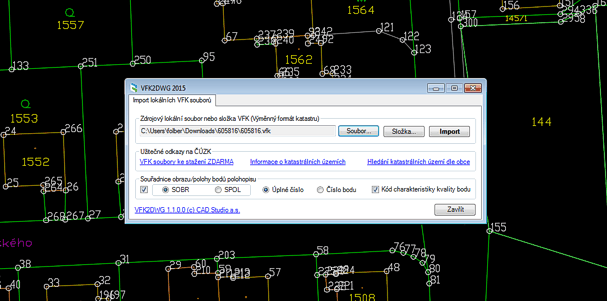
\includegraphics[width=14cm]{./pictures/vfk2dwg.png}
      \caption{Import VFK souborů (zdroj:
\href{http://www.cadstudio.cz/img/vfk2dwg11.gif}{cadstudio.cz})}
      \label{fig:cadstudio}
  \end{figure}
%http://www.cadstudio.cz/vfk2dwg
\end{itemize}
\subsection{knihovna GDAL}
\label{subsec:gdal_vfk}
VFK Driver je součástí knihovny \zk{GDAL} a umožňuje čtení souborů výměnného formátu katastru nemovitostí(VFK). Driver, česky ovladač, slouží obecně k rozšíření funkcionality. Soubor \zk{VFK} je driverem vnímán jako zdroj dat(\verb|OGR datasource|) s žádnou nebo více vrstvami(\verb|OGR layers|). Body jsou ve vrstvách reprezentovány jako \verb|wkbPoints|, linie a hranice jako \verb|wkbLineStrings| a plochy jako \verb|wkbPolygons|. VFK driver si během prvního čtení ukládá data do SQLite databáze, která se vytvoří ve stejném adresáři jako je vfk soubor. Opakované načtení je díky již vytvořené databázi výrazně rychlejší. Výhoda databáze je v snazším a rychlejším přístupu k datům. Dále si může uživatel pomocí systémových proměnných \verb|OGR_VFK_DB_OVERWRITE| a \verb|OGR_VFK_DB_NAME| nastavit jestli bude vytvořená SQL databáze při opakovaném načtení přepsána(čtení stále z vfk souboru) a jaký bude název vytvořené databáze. Navíc je tento driver jako jediný z výše zmíněných nástrojů volně dostupný. \cite{vfk_driver}

\begin{figure}[H]
	 \centering
      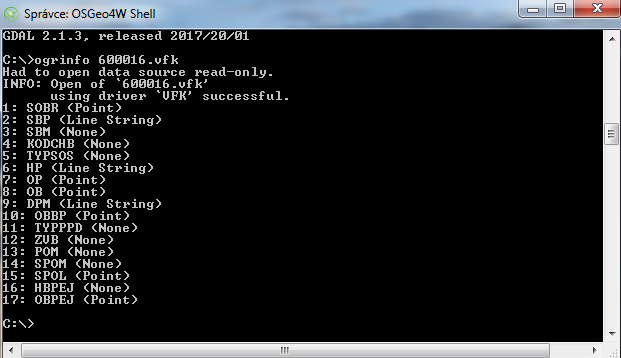
\includegraphics[width=15cm]{./pictures/vfk_driver.png}
      \caption{Ukázka použití VFK driveru (zdroj:vlastní)}
      \label{fig:vfk_driver}
  \end{figure}
%zdroj:http://gdal.org/drv_vfk.html
%http://freegis.fsv.cvut.cz/gwiki/VFK_/_GDAL
%http://freegis.fsv.cvut.cz/gwiki/V%C3%BDm%C4%9Bnn%C3%BD_form%C3%A1t_ISKN
%VFK/QGIS plugin
%http://freegis.fsv.cvut.cz/gwiki/VFK_/_QGIS_plugin
\section{Sestavení geometrie prvků}
\label{sec:sestaveni_geometrie}
Po načtení \zk{VFK} souboru VFK Driverem(\ref{subsec:gdal_vfk}) nedojde k sestavení geometrie prvků automaticky pokud je verze knihovny GDAL 2.1 a nižší. Uživatel si proto musí o sestavení geometrie sám říct dotazem na požadovanou geometrii, například chceme-li geometrii bloku HP: \textbf{GetLayerByName('HP').GetFeature(1)}. Geometrie se sestavuje postupně po blocích dle schématu počínaje blokem SOBR(souřadnice obrazu bodů polohopisu):
\begin{figure}[H]
	 \centering
      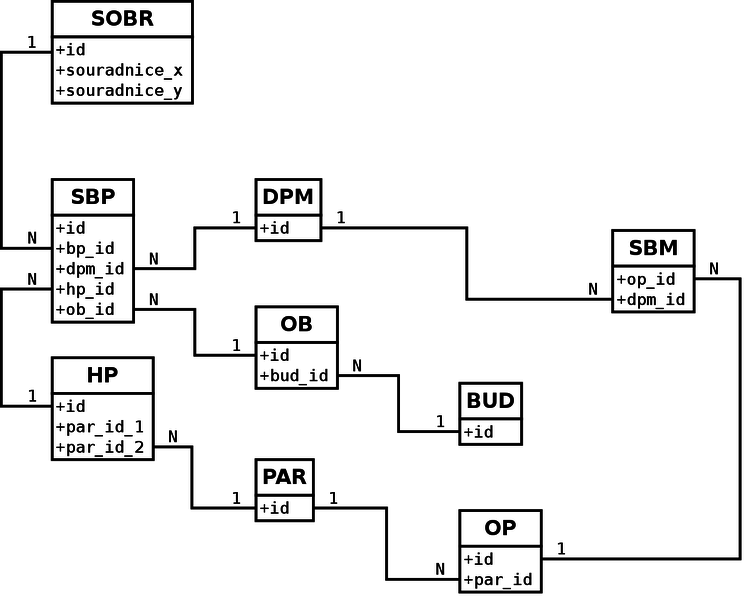
\includegraphics[width=10cm]{./pictures/Vfk-diagram-geom.png}
      \caption{Přehled datových bloků pro sestavení geometrie prvků digitální katastrální mapy (zdroj:
      \href{http://freegis.fsv.cvut.cz/wiki/images/thumb/8/8a/Vfk-diagram-geom.png/744px-Vfk-diagram-geom.png}{freegis.fsv.cvut.cz})}
      \label{fig:vfk_diagram_geom}
  \end{figure}
Pokud má být sestavena geometrie bloku HP(hranic parcel), dojde po provedení dotazu na geometrii hranic parcel k sestavení geometrie i všech předchozích bloků. Výsledkem dotazu je tedy sestavená geometrie nejen pro blok hranic parcel, ale také pro blok SOBR(souřadnice obrazu bodů polohopisu) a blok SBP(spojení bodů polohopisu). Geometrie datového bloku HP je pro tuto práci důležitá, protože právě z ní dojde k sestavení bloku PAR(parcely). Stejně tak datový blok SBP, který bude využit k sestavení bloku BUD(budovy).
%zdroj: http://freegis.fsv.cvut.cz/gwiki/VFK_/_GDAL
\chapter{Použité technologie}
\label{3-technologie}
%% ML: programy -> technologie (ci neco vice obecneho nez programy)
%% LK: -> technologie
V této kapitole budou zmíněny technologie, které byly pro tvorbu
bakalářské práce využity. Patří sem hlavně programovací jazyk Python,
%% ML: plugin vznika? zkuste preformulovat
%% LK: preformulovano jiz driv, jen pro poradek :-)
geografický informační systém QGIS, pro který je zásuvný modul vyvíjen.
%% ML: posledni vete vubec nerozumim, orientaci? Mate na mysli, to ze
%% jste pouzival Qt Creator pro tvorbu UI? Qt je graficky framework na
%% kterem je QGIS postaven.
%% LK: mel jsem na mysli Qt creator,zminim zde Qt
%% ML: OK
Pro práci důležitou technologií je i knihovna GDAL a grafický
framework\footnote{Softwarová struktura sloužící jako podpora při
  vývoji nových programů} Qt.

\section{Python}
\label{sec:python}
\begin{figure}[H]
	 \centering
      
\includegraphics[width=5cm]{./pictures/python-logo.png}
      \caption{Logo Python (zdroj:
\href{https://www.python.org/static/community_logos/python-logo-master-v3-TM.png}{Python.org})}
      \label{fig:python}
  \end{figure}

%% ML: druhou cast souveti prepiste anebo uplne vynechte
%% LK: vynechána
%% ML: dobre
Za autora programovacího jazyka Python je považován Guido vam Roosum.
%% ML: drou vetu prepiste do cestiny, pocatek ... byl ... na
%% LK: prepsano
Počátek vývoje jazyka Python byl v roce 1990 na Stichtig Mathematisch
Centrum v Nizozemí. Hlavní princip
%% ML: osloveni Guido zni familiarne, odkud jste text cerpal?
%% LK: cerpano je z ucebnice jazyka Python, odkaz {ucebnicepython},
%% odkaz na zdroj presunut z konce textu pod tento odstavec
vychází z programovacího jazyka ABC. Python je volně dostupný včetně
standardních knihoven, dokumentace a zdrojových kódů. V roce 2001
vznikla nezisková organizace Python Software Foundation, která je
vlastníkem veškerých intelektuálních materiálů souvisejících s
programovacím jazykem
%% ML: poznamka pod carou: velmi zjednodusena definice open source
%% ML: lepsi
%% LK: ok
Python. Spravuje open source\footnote{Jedná se o technologie s volně
  poskytovanými zdrojovými kódy, na vývoji se tak může podílet
  kdokoliv} licence Pythonu od verze 2.1 a výš. Zároveň se stará o
%% ML: posledni veta (pod), ktera se na vyvoji jazyka take podilela a pod...
%% ML: zbytek vety jsem odstranil
%% LK: ok
ochranou známku jazyka. Jedním ze sponzorů neziskové organizace je
společnost Digital Creations. \cite{ucebnicepython}

Python účinně a efektivně pracuje s vysokoúrovňovými datovými
typy. Syntaxe jazyka a dynamické typy z něj dělají vhodný nástroj pro
%% ML: mate v seznamu zkratek?, zde nemate rozepsanu
%% LK: ano mam
%% ML: OK
psaní skriptů a rychlý vývoj aplikací (\zk{RAD}). Jazyk si snadno
%% ML: cteni syntaxe nezni cesky,..
%% LK: prepsano
oblíbí začátečníci, pro které je struktura jazyka snadno pochopitelná. 
%% ML: co znamena ``interpret''
%% LK: myslel jsem opreacni systemy
%% ML: v poradku
Další výhodou je spustitelnost na velkém množství operačních systémů
zahrnujících Linux, Windows, MacOS. \cite{python, diveintopython}

%obrazek: https://www.raspberrypi.org/documentation/usage/python/images/python-logo.png
%zdroje:https://docs.python.org/3/tutorial/index.html a https://i.iinfo.cz/files/root/k/Ucebnice_jazyka_Python.pdf
\section{QGIS}
\label{sec:qgis}
\begin{figure}[H]
	 \centering
      
\includegraphics[height=4cm]{./pictures/qgis-logo.jpg}
      \caption{Logo QGIS (zdroj:
\href{https://euipo.europa.eu/copla/image/CJ4JX4FZVCC523YA2TMALSKFLFPOWZHPVHYMP5QREVP2BOXHB3PCM7RCOZR6TEIMWNCQDAB6N25VA}{qgis.org})}
      \label{fig:qgis}
  \end{figure}
  
  Jedná se o volně dostupný geografický informační systém (\zk{GIS}),
  který slouží pro práci s geodaty\footnote{Data s prostorovou a
    atributovou složkou, která se vztahují ke konkrétnímu místu na
  %% ML: druhou vetu prepiste, aby znela vice cesky
  %% LK: veta zjednodusena
    %% ML: OK
   Zemi.}. Licenci k programu má ve správě GNU General Public
License. QGIS je oficiálním projektem Open Source Geospatial
Foundation(\zk{OSGeo}) a je spustitelný na nejužívanějších operačních
systémech jako Windows, Linux, Mac\-OS. Samotný systém je napsaný v
jazyce C++ a jeho výhodou je velké množství nejrůznějších rozšíření
(zásuvných modulů), které je možné snadno doinstalovat. Zásuvné moduly
mohou být napsané nejen v C++, ale také v programovacím jazyce
Python. QGIS podporuje mnoho formátů -- rastrových,
vektorových i databázových. Aktuálně nejnovější verze je 2.18.15
nazvaná \textit{Las Palmas} a vydaná dne 8.12.2017.

Vývoj systému začal roku 2002 Garym Shermanem, ještě pod názvem
\textit {Quantum GIS} (toto označení zůstalo až do verze 2.0).\cite{qgis_official, qgis_wiki_en, qgis_wiki_cz}
%% ML: tuto informaci mate na zacatku odstavce, staci jednou
%% LK: odstraneno
%% ML: OK
 
%zdroj: https://www.qgis.org/en/site/, https://cs.wikipedia.org/wiki/QGIS, https://en.wikipedia.org/wiki/QGIS
%obrazek: https://euipo.europa.eu/copla/image/CJ4JX4FZVCC523YA2TMALSKFLFPOWZHPVHYMP5QREVP2BOXHB3PCM7RCOZR6TEIMWNCQDAB6N25VA
\section{QGIS VFK Plugin}
\label{sec:qgis_plugin}
\begin{figure}[H]
	 \centering
      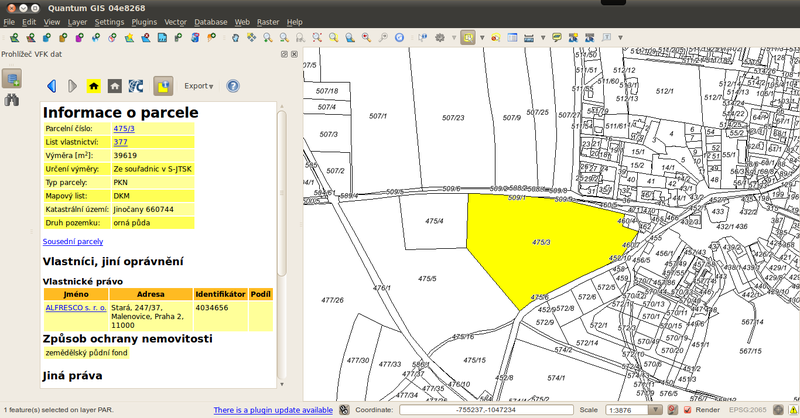
\includegraphics[height=5cm]{./pictures/Qgisvfkplugin.png}
      \caption{Ukázka prostředí pluginu (zdroj:
        %% ML: freegis.fsv.cvut.cz
        %% LK: opraveno
\href{http://freegis.fsv.cvut.cz/wiki/images/4/4b/Qgisvfkplugin-screenshot-05.png}{freegis.fsv.cvut.cz})}
      \label{fig:qgis_vfk_plugin}
  \end{figure}

Jde o zásuvný modul (anglicky plugin) pro geografický informační systém
%% ML: predlozka ``z'' neni v tomto kontextu moc vhodna
%% ML: predlozky mate v textu naduzivany a casto ve spatne kontextu (pod/z)
%% LK: na predlozky se zamerim 
QGIS, který umožňuje práci s daty českého katastru
%% ML: na tomto miste bych nepouzival ``uplne'', pro plugin je
%% podstatne, aby se v datech vyskytovali bloky PAR a BUD (skupina
%% NEMO), jinak nemusi byt '``uplna''
%% LK: odstraneno uplnymi, mám zmínit, že data musí obsahovat datovou skupinu NEMO?
%% ML: ano, muzete zminit
%% LK: zmineno
nemovitostí. Zásuvný modul pracuje s daty v takzvaném novém
výměnném formátu katastru, který je označovaný \zk{VFK} nebo
\zk{NVF}. Data ze souboru, který musí obsahovat datovou skupinu NEMO, jsou čtena pomocí knihovny \zk{GDAL}. Plugin
%% ML: Pri cem jinem? ;-) Zkuste preformulovat
%% LK: preformulovano :)
%% ML: OK
umožňuje vyhledávání a zobrazování informací z načtených dat katastru
nemovitostí. Ovládání je uživatelsky přívětivé a známé vzhledem k
podobnému rozhraní jako je u webových aplikací.

%% ML: nyni?
%% LK: zmenen zacatek vety
%% ML: OK
V aktuální verzi je možné pro nahraná data vyhledávat: parcely, budovy, jednotky
a oprávněné osoby. Prohlížeč dat umožňuje zobrazit list vlastnictví a
další výpisy informací: o parcele, o budově, o jednotce a o oprávněné
osobě. Dále prohlížeč umožňuje zobrazení aktuálního stavu nemovitosti
na stránkách Nahlížení do katastru nemovitostí a export výpisů do
formátů HTML a zdrojového kódu LaTeXu (možnost vytvoření PDF a
PS\footnote{Programovací jazyk PostScript vyvinutý ke grafickému
  popisu tisknutelných dokumentů, výhodou je nezávislost na zařízení,
  ze kterého se tiskne, podobně jako formát PDF. \cite{PostScript}}).

%% ML: Obe vety zacinaji temer stejne: Zdrojove kody/texty, zkuste prepsat
%% ML: v poradku
Zdrojové kódy zásuvného modulu jsou ke stažení na adrese
\href{https://github.com/ctu-geoforall-lab/qgis-vfk-plugin}{Git
  repozitáře} a jsou šířeny pod licencí
\href{https://raw.githubusercontent.com/ctu-osgeorel/qgis-vfk-plugin/master/LICENSE}{GNU
  GPL}.

První verze zásuvného modulu (verze1.x) byla napsána v jazyce C++ a vyvinuta studenty
oboru Geoinformatika Annou Kratochvílovou a Václavem Petrášem na FSv
ČVUT v Praze v roce 2012. Druhá verze 2.x byla vyvíjena v letech 2015
a 2016 studentem stejného oboru Štěpánem Bambulou a zásuvný modul byl
přepsán do jazyka Python. \citep{vfk_qgis_plugin}
%http://freegis.fsv.cvut.cz/gwiki/VFK_/_QGIS_plugin
%https://cs.wikipedia.org/wiki/PostScript
 
\section{GDAL}
\label{sec:gdal}
\begin{figure}[H]
	 \centering
      
\includegraphics[height=5cm]{./pictures/gdal-logo.png}
      \caption{Logo GDAL (zdroj:
\href{https://upload.wikimedia.org/wikipedia/commons/thumb/d/df/GDALLogoColor.svg/572px-GDALLogoColor.svg.png}{gdal.org})}
      \label{fig:gdal}
  \end{figure}
  
Geospatial Data Abstraction Library (GDAL) je knihovna určená pro čtení
a zápis vektorových a rastrových formátů geodat. Jde o open source
vyvíjený pod licencí X/MIT a jako součást projektu Open Source
Geospatial Foundation (\zk{OSGeo}). Samotná knihovna je reprezentována
jedním abstraktním modelem pro rastrová data a jedním pro vektorová
data. Dále knihovna nabízí užitečné nástroje pro příkazovou řádku,
které slouží ke konverzi a zpracování dat. Od verze GDAL 2.0 je
součástí knihovny GDAL také knihovna OGR, která zajišťuje
funkcionalitu jednoduchých prvků vektorových dat.

Nejdříve byla knihovna vyvíjena Frankem Warmerdamem, od verze 1.3.2
došlo k převedení na GDAL/OGR Project Management Committee, který je
součástí \zk{OSGeo}. Knihovna je díky velké funkcionalitě často
využívána v komerční i nekomerční sféře a proto patří v \zk{GIS} mezi
hlavní volně dostupné softwary. \cite{gdal, gdal_wiki}
%obrazek: https://upload.wikimedia.org/wikipedia/commons/thumb/d/df/GDALLogoColor.svg/572px-GDALLogoColor.svg.png
%zdroje: http://www.gdal.org/, https://cs.wikipedia.org/wiki/GDAL

\section{Qt}

\begin{figure}[H]
	 \centering
      
\includegraphics[width=3cm]{./pictures/qt-logo.png}
      \caption{Logo Qt (zdroj:
\href{https://upload.wikimedia.org/wikipedia/commons/thumb/0/0b/Qt_logo_2016.svg/578px-Qt_logo_2016.svg.png}{wikipedia.org})}
      \label{fig:qt}
  \end{figure}

  %% ML: chybi Vam tu kontext: na tomto grafickem frameworku je postaven QGIS!
  %% ML: v poradku
  Qt je multiplatformní aplikační rámec (framework), který je určen
  pro vývoj aplikačního softwaru. Ten může snadno fungovat na různých
  platformách s žádnými nebo jen minimálními změnami v kódu. QGIS (viz
  kap. \ref{sec:qgis}) samotný je na tomto grafickém aplikačním rámci
  postaven. Qt je aktuálně vyvíjen společnostmi \textit{The Qt
    Company} a \textit{Qt Project}.\cite{qt_wiki, qt}

%zdroj: https://en.wikipedia.org/wiki/Qt_(software)
%obrazek: https://upload.wikimedia.org/wikipedia/commons/thumb/0/0b/Qt_logo_2016.svg/578px-Qt_logo_2016.svg.png


\chapter{Knihovna publicvfk}
\label{4-plugin}
Tato kapitola bude věnována informacím o nové knihovně \textbf{publicvfk} pro zásuvný modul \textit{QGIS VFK Plugin} a její integraci do zásuvného modulu. Bude popsána funkčnost knihivny, uvedeno co je pro knihovnu vstupem a co výstupem. Dále bude ukázána funkčnost na testovacích datech a doplněny informace o způsobu integrace do výše zmíněného zásuvného moudlu \textit{QGIS VFK Plugin}. Pro tvorbu bylo čerpáno ze zdrojů \cite{cookbook, ucebnicepython}.

\section{Funkčnost knihovny}
\label{sec:funknost_knihovny}
Knihovna načte pomocí VFK driveru(\ref{subsec:gdal_vfk}) textový soubor ve formátu \zk{VFK}, čímž vznikne SQL databáze s načtenými daty. \zk{VFK} soubor již není dále využíván, knihovna místo toho přistupuje k vytvořené databázi. Dále je zkontrolována verze knihovny GDAL, která když není vyšší než 2.2, tak musí být proveden příkaz \verb|self.dsn_vfk.GetLayerByName('HP').GetFeature(1)|, díky kterému dojde k sestavení geometrie všech datových bloků před blokem hranic parcel(HP), viz.\ref{sec:sestaveni_geometrie}.

Pro správné fungování při načítání dat z databáze je nezbytné přidat do databáze tabulku geometrie (\verb|geometry columns|) a tabulku souřadnicového systému (\verb|spatial_ref_sys|). Dojde tak k vytvoření prostorové databáze\footnote{Databáze ukládající prostorovou složku dat.}. SQLite driver bez tabulek nerozezná datový typ vrstev. Novější verze knihovny si s absencí tabulek dokáže poradit, resp už si tabulky vytváří sama.

Po vytvoření prostorové databáze následuje postupně vytvoření tabulky s názvem PAR pro parcely, sestavení a zapsání geometrie parcel i s atributy, vytvoření tabulky s názvem BUD pro budovy a sestavení a zapsání geometrie budov včetně atributů.

Pro sestavení geometrie parcel je využito datového bloku HP (Hranice parcel), kde je možné pomocí atributů \verb|PAR_ID_1| a \verb|PAR_ID_2|(\ref{subsec:bloky_par_bud}) zjistit seznam všech parcel a příslušné hranice jedné parcely. Samotná geometrie parcel je sestavená geometrickou cestou, tedy postupným sestavováním hranici po hranici parcelu po parcele. Následující pseudokód(\ref{alg:sestaveni_parcely}) popisuje proces sestavení a uložení geometrie parcel. Na řádku 10 je volána metoda \verb|build_bound()|(\ref{subsec:sestaveni_geometrie}) pro sestavení samotné geometrie, jejíž princip je znázorněn diagramem v příloze \ref{fig:logika_geometrie}.

\begin{algorithm}
\caption{Logika sestavení a uložení geometrie parcel}
\label{alg:sestaveni_parcely}
	\begin{algorithmic}[1]
	\STATE{číslaParcel = zjisti SQL příkazem unikátní čísla parcel}
	\STATE{NeuzavřenéParcely = prázdný seznam}
	\STATE{Začátek transakce}
	\FOR{Parcela \textbf{in} číslaParcel}
		\STATE{seznamGeometriíHranice = prázdný seznam}
		\FOR{prvek \textbf{in} filtrVrstvy(vrstva = HraniceParcel, filtr = Parcela)}
			\STATE{geometrie = geometrie prvku}
			\STATE{přidej geometrie do seznamGeometriíHranice}
		\ENDFOR
		\STATE{polygonGeometrie = sestav geometrii ze seznamGeometriíHranice}
		\IF{polygonGeometrie \textbf{is not} prázdný}
			\STATE{převeď polygonGeometrie do roviny(2D)}
		\ELSE
			\STATE{Přidej číslo parcely do NeuzavřenéParcely}
		\ENDIF
		\STATE{Vytvoř nový řádek tabulky}
		\STATE{Nastav geometrii sestavované parcely do nového řádku}
		\STATE{Nastav hodnotu do sloupce \verb|"id_par"| pro nový řádek}
		\STATE{Nastav hodnotu do sloupců \verb|"kmenove_cislo_par"|, \verb|"poddeleni_cisla_par"| pro nový řádek}
		\STATE{Přidej nově vytvořený řádek do tabulky}
	\ENDFOR
	\STATE{Konec transakce}
	\end{algorithmic}
\end{algorithm}

K sestavení geometrie budov je využit datový blok SBP (spojení bodů polohopisu) a blok OB (obrazy budov). Nejprve jsou zjištěna z bloku OB unikátní identifikační čísla budov včetně příslušných identifikačních čísel hranic budov, pro které je následně vyhledána geometrie v tabulce SBP. Sestavení geometrie budov probíhá také geometrickou cestou. Logika sestavování geometrie je znázorněna diagramem v příloze, viz. \ref{fig:logika_geometrie}.
%zdroj: http://gdal.org/drv_sqlite.html

\section{Vstupní data}
Vstupními daty pro knihovnu je textový soubor ve formátu \zk{VFK} s neúplnými daty(\ref{subsec:neuplna_data}). Knihovna přebírá adresu vstupního souboru, dochází k načtení dat a zápisu do databáze.

\subsection{Testovací data}
Zkomprimovaná testovací data ve formátu VFK byla stažena pro katastrální území Abertamy na adrese: \href{http://services.cuzk.cz/vfk/ku/20170901/600016.zip}{http://services.cuzk.cz/vfk/ku/20170901/600016.zip}.
{\scriptsize
\begin{lstlisting}[caption=Ukázka bloku hranic parcel(HP) -- definice bloků a věty dat(zdroj:vlastní), label=lst:data]
&BHP;ID N30;STAV_DAT N2;DATUM_VZNIKU D;DATUM_ZANIKU D;PRIZNAK_KONTEXTU N1;
RIZENI_ID_VZNIKU N30;RIZENI_ID_ZANIKU N30;TYPPPD_KOD N10;PAR_ID_1 N30;PAR_ID_2 N30
&DHP;3491827403;0;"07.04.2009 08:59:39";"";3;1991606403;;21900;706860403;708070403 
&DHP;3491828403;0;"07.04.2009 08:59:39";"";3;1991606403;;21900;706860403;708070403
&DHP;3491829403;0;"07.04.2009 08:59:39";"";3;1991606403;;21900;706860403;708070403
&DHP;3491830403;0;"07.04.2009 08:59:39";"";3;1991606403;;21900;706860403;708070403
&DHP;3491831403;0;"07.04.2009 08:59:39";"";3;1991606403;;21900;706860403;708070403
\end{lstlisting}}
Na řádcích 1-2~(\ref{lst:data}) je rozdělený uvozovací řádek datového bloku HP(hranic parcel).Řádky 3-7~(\ref{lst:data}) představují věty dat, ve kterých jsou uložena vlastní data ve stanoveném pořadí.
\subsection{Funkčnost knihovny s testovacími daty}
Databáze sice obsahuje datové vrstvy, ale SQL driver není schopen je rozeznat, proto mají všechny hodnotu None. Zároveň databáze neobsahuje bloky parcel a budov.
\begin{figure}[H]
	 \centering
      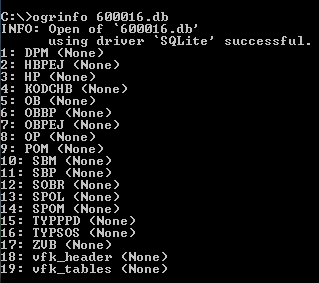
\includegraphics[height=5cm]{./pictures/funkcnost_knihovny_pred.png}
      \caption{Databáze před použitím knihovny(zdroj:vlastní)}
      \label{fig:funkcnost_pred}
\end{figure}
Po použití knihovny SQL driver rozezná díky přidaným tabulkám datové bloky. Databáze již obsahuje sestavené bloky parcel \textbf{PAR(Polygon)} a budov \textbf{BUD(Polygon)}. 
\begin{figure}[H]
	 \centering
     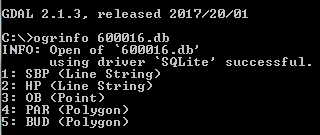
\includegraphics[height=3cm]{./pictures/funkcnost_knihovny_po.png}
     \caption{Databáze po použití knihovny(zdroj:vlastní)}
     \label{fig:funkcnost_po}
\end{figure}  
  
\section{Výstupní data}
Výstupem k knihovny je sestavená geometrie pro bloky parcel a budov. Geometrie je společně s dalšími hodnotami jako je identifikační číslo, číslo parcely zapsána do VFK Driverem\ref{subsec:gdal_vfk} vytvořené databáze.

\section{Popis tříd knihovny a jejich metod}
\label{sec:popis_trid}
V této podkapitole budou představeny jednotlivé třídy knihovny, jejich členské metody a popsáno, co která třída a metoda obstarává.

\subsection{VFKBuilderError}
Tato třída dědí vlastnosti třídy Exception a je volána v případě, že nastane chyba. To se může stát není-li připojen \zk{VFK} souboru nebo databáze.
\subsection{VFKBuilder}
\label{subsec:sestaveni_geometrie}
Mateřská třída, která obsahuje společné metody tříd VFKParBuilder a VFKBudBuilder určených pro sestavení geometrie parcel i budov.
\begin{itemize}[leftmargin=50pt]
\item \verb|__init__()|
		
V konstruktoru třídy dochází k vytvoření tabulky geometrie (\verb|geometry columns|) a tabulky souřadnicového systému (\verb|spatial_ref_sys|), bez kterých by nebylo možné číst geometrii z databáze. V případě nepřipojeného zdroje dat - \zk{VFK} souboru, je volána třída VFKBuilderError a zobrazena chybová hláška.
\item \verb|build_bound()|

Hlavních metod, která sestavuje geometrii jednotlivých hranic. V případě hranice s dírami dojde k vytvoří seznamu s více geometriemi, ve kterém je nalezena největší a ze zbylých geometrií jsou vytvořeny díry. Sestavení probíhá geometrickou cestou. Nejdříve je přidána první hranice, poté hranice co začíná koncovým bodem první hranice a tak dokola. Na závěr je otestováno uzavření všech hranic v seznamu geometrií(první bod hranice je shodný s posledním bodem hranice).
\item \verb|add_boundary()|

Metoda pro přidávání jedné hranice do geometrie. Přidávání hranice probíhá bod po bodu a přidaná hranice je ze seznamu hranic po přidání do geometrie odstraněna, aby se seznam zmenšil. Všechny hranice nemají stejnou orientaci(některé na sebe navazují koncovými body), tudíž je potřeba body hranice přidávat "odzadu".
\item \verb|filter_layer()|

Na základě specifikovaného atributového filtru a názvu datového bloku vrací výsledné hodnoty uložené v seznamu.
\item \verb|executeSQL()|

Provadí sql dotaz v databázi a vrací výsledek uložený do seznamu.

\end{itemize}
\subsection{VFKBudBuilder}
Potomek třídy \textbf{VFKBuilder}. Třída sestavuje geometrii budov a ukládá ji do nově vytvořené tabulky BUD v databázi. Ukládání probíhá v transakci.
\begin{itemize}[leftmargin=50pt]
\item \verb|__init__()|

Konstruktor třídy, kde je vytvořena nová tabulka pro budovy -- BUD a atribut \verb|id_bud|.
\item \verb|build_all_bud()|

Metoda se stará o sestavení všech nebo jen části budov. To je možné nastavit parametrem limit. Po sestavení probíhá v transakci uložení geometrií a atributů do tabulky BUD v databázi.
\end{itemize}
\subsection{VFKParBuilder}
Potomek třídy \textbf{VFKBuillder}. V této třídě dochází k samotnému sestavení geometrie parcel, vytvoření nové tabulky PAR v databázi a zapsání dat. Zapisuje se identifikační číslo parcely(\verb|par_id|), kmenové číslo parcely(\verb|kmenove_cislo_par|), poddělení čísla parcely(\verb|poddeleni_cisla_par|) a samozřejmě geometrie dané parcely. Zápis do databáze je proveden v transakci, čímž je zaručené korektní zapsání všech parcel nebo žádné -- v případě chyby.

\begin{itemize}[leftmargin=50pt]
\item \verb|__init__()|

Konstruktor třídy, kde je vytvořena nová tabulka pro parcely -- PAR včetně atributů.
\item \verb|build_all_par()|

Zde probíhá samotné sestavení všech parcel. Po sestavení je parcela uložena do databáze i s příslušnými atributy. Metodě je možné nastavit kolik parcel má sestavit. Základně dochází k sestavení všech parcel.

\end{itemize}
\section{Integrace knihovny do zásuvného modulu}
\label{sec:integrace_knihovny}
Základem integrace bylo správné umístění do kódu zásuvného modulu, přesněji do souboru \textit{mainApp.py}. Bylo potřeba zachovat funkcionalitu při otevření úplných i neúplných dat. Jsou-li data úplná, funguje zásuvný modul standardně. Pokud data neobsahují bloky PAR a BUD -- jsou neúplná, dojde k jejich sestavení a tedy zavolání třídy z nově integrované knihovny \textbf{publicvfk}.

Nejdříve je knihovna pomocí metody import nahrána. Dále je ve funkci \textbf{loadVfkFile()} proveden test na přítomnost bloku parcel('PAR') pomocí metody GetLayerName():
\begin{lstlisting}[language=Python, numbers=none]
t_par = self.__mOgrDataSource.GetLayerByName('PAR')
\end{lstlisting}
Předpokladem je, že bloky parcel a budov jsou v datech obsaženy oba nebo žádný, proto je testována jen přítomnost bloku parcel. Není-li blok obsažen, dojde k uzavření zdroje dat:
\begin{lstlisting}[language=Python, numbers=none]
self.__mOgrDataSource = None
\end{lstlisting}
, aby mohlo proběhnout sestavení bloků. Knihovna si vytváří vlastní připojení k \zk{VFK} souboru a databázi, proto je třeba zdroj dat uzavřít a předejít tak zdvojenému připojení k \zk{VFK} souboru či databázi. Vícenásobné připojení může způsobit chybu. Následuje sestavení neobsažených bloků parcel a budov z knihovny \textbf{publicvfk}. O sestavení parcel se postará třída \textit{VFKParBuilder} a o sestaveni budov třída \textit{VFKBudBuilder}. Nejprve jsou deklarovány objekty dané třídy a následně jsou volány metody pro sestavení geometrií:

\begin{lstlisting}[language=Python, numbers=none]
# Build Parcels
parcels = VFKParBuilder(fileName)
parcels.build_all_par()
# Build Buildings
buildings = VFKBudBuilder(fileName)
buildings.build_all_bud()
\end{lstlisting}

Po sestavení bloků parcel a budov je zdroj dat pomocí proměnné prostředí nastaven na databázi, která vznikne o adresář výš při otevření \zk{VFK} souboru a nese jméno \zk{VFK} souboru, kde je místo přípony \verb|.vfk| přípona \verb|_stav.db|:
{\small
\begin{lstlisting}[language=Python, numbers=none]
self.__mOgrDataSource = ogr.Open(os.environ['OGR_VFK_DB_NAME'], 0)
self.__mDataSourceName = os.environ['OGR_VFK_DB_NAME']
\end{lstlisting}}
%self.__mDataSourceName = os.environ['OGR_VFK_DB_NAME'] PROČ, nastavuje zde taky prostredi? 

V této databázi jsou uložena data z načtení \zk{VFK} souboru a také knihovnou vytvořené tabulky s bloky PAR a BUD. Zásuvný modul z této databáze čerpá data.

Při načítání neúplných dat \zk{VFK} může nastat situace, kdy už jsou tabulky parcel a budov nebo jen jednoho bloku v databázi zapsané. SQL driver však bloky nedokáže rozeznat, protože databáze není prostorová, viz.\ref{sec:funknost_knihovny}. Pro tento případ je v knihovně před vytvářením jednotlivé tabulky testováno, jestli databáze blok parcel nebo budov opravdu neobsahuje. Tento test je v kódu umístěn až za přidáním tabulek s geometrií a souřadnicovým systémem, tudíž je nepřítomnost zapsaných dat vyloučena. Zjistí-li se po přidání tabulek, že jsou oba datové bloky -- parcely a budovy v databázi již zapsané, knihovna sestavení neprovede. 
\section{Testování knihovny}
Funkčnost knihovny je možné otestovat z příkazové řádky. K testování byl využit modul sys, který je obsažen v základní distribuci Pythonu a díky kterému je možné realizovat množství úloh spojených s interpretrem. Příkaz pro spuštění se skládá z názvů knihovny a \zk{VFK} souboru včetně přípony, oddělených mezerou. Například: \textit{python publicvfk.py 600016.vfk}, viz. \ref{fig:testovani_ukazka}. Jméno knihovny a další argumenty(v našem případě název \zk{VFK} souboru) předané z příkazové řádky jsou uloženy v proměnné \textit{sys.argv}, která se chová jako seznam.

\begin{figure}[H]
	 \centering
      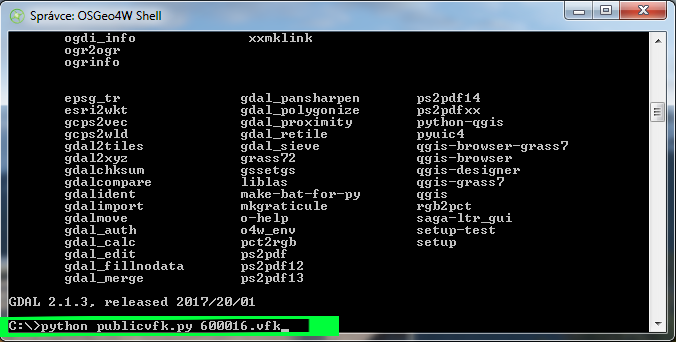
\includegraphics[height=7cm]{./pictures/testovani_ukazka.png}
      \caption{Ukázka testovacího spuštění knihovny}
      \label{fig:testovani_ukazka}
  \end{figure}

Zadání názvu knihovny i názvu \zk{VFK} souboru současně kontroluje podmínka(\ref{lst:chyba}),pokud je spuštění knihovny nekorektní je interpretr ukončen a zobrazena chybová hláška(\ref{fig:testovani_hlaska}).
\begin{lstlisting}[caption=Podmínka pro spouštěcí příkaz, language=Python, label=lst:chyba, numbers=none]
    if len(sys.argv) != 2:
        sys.exit("{} soubor.vfk".format(sys.argv[0]))
\end{lstlisting}

\begin{figure}[H]
	 \centering
      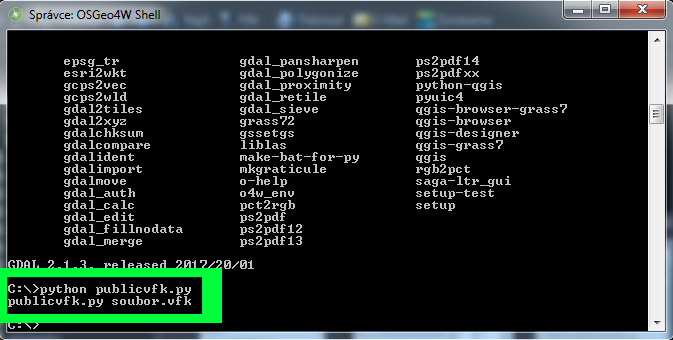
\includegraphics[height=7cm]{./pictures/testovani_hlaska.png}
      \caption{Chybová hláška včetně nekompletního příkazu při nesprávném použití knihovny}
      \label{fig:testovani_hlaska}
  \end{figure}

Testování je možné jen při přímém spuštění knihovny, nikoli je-li knihovna importována jako modul. K tomu je využita speciální proměnná \verb|__name__|, do které je interpretrem v případě spuštění přímo uložena hodnota \verb|"__main__"| a podmínka je splněna(viz.\ref{lst:podminka}). Je-li knihovna importována z jiného modulu je proměnná \verb|__name__| nastavena na jméno modulu a podmínka není splněna.
\begin{lstlisting}[caption=Ukázka sestavení bloků provedeném jen při přímém spuštění knihovny, language=Python, numbers=none, label=lst:podminka]
if __name__ == "__main__":
	#Sestaveni bloku primo z knihovny
    parcel = VFKParBuilder(sys.argv[1])
    parcel.build_all_par()
    building = VFKBudBuilder(sys.argv[1])
    building.build_all_bud()
\end{lstlisting}
%ucebnice jazyka Python str 10
\chapter{Závěr}
\label{5-zaver}
%Shrnutí cíle práce

%% ML: vyskrtnete ``moji'', jasne veci neni treba opakovat
%% LK: to je :-)
%% ML: odstavec - jedno ohromne souveti, prepiste...
%% LK: prepisu
%% ML: jeste se na ten odstavec podivejte, ve vsech vetam mluvite o "rozsireni"
%% ML: zkuste jeste jednou odstavec projit a preformulovat, zaver by mel byt nejlepsi casti praci
%% LK: pomuze slovo vylepsit?
%% ML: treba, pro urychleni jsem prepsal, v druhe vete treba Upraveny
%% ML: vylepsovany jsem odstranil
Cílem bakalářské práce bylo vytvoření nové knihovny napsané v jazyce
Python a~vylepšit tak funkcionalitu stávajícího zásuvného modul QGIS
pro práci s katastrálními daty. Zásuvný modul umožňuje práci
pouze se zpoplatněnými českými katastrálními daty ve formátu
\zk{VFK}. Nové rozšíření mělo navíc umožňovat načítání neúplných
veřejně dostupných dat výměnného formátu katastru nemovitostí a
sestavení bloků parcel a budov z načtených dat.

% Upřesněný výsledek
%% ML: prvni a druha veta rika to same, prepiste
%% LK: prvni vetu dam pryc
Podařilo se vytvořit takovou knihovnu, která
splňuje výše zmíněné zadání.
%% ML: druha veta opakuje to co jiz bylo receno, preformulujte
%% LK: preformulovano
%% ML: neuplne -> verejne dostupne (tj. data bez bloku NEMO - pokud si dobre vzpominam)
%% LK: opraveno
Veřejně dostupná data neobsahují datovou skupinu Nemovitosti, ve které
jsou obsaženy bloky parcel a budov. Proto knihovna oba bloky sestavuje
%% ML: proc je to nutne? -> vizualizace dat v pluginu, nevim, zda to
%% mate nekde jasne receno, minimalne, zde by to melo byt ucineno
%% LK: dopsano
%% ML: lepsi
a ukládá je do databáze, která vznikne při načtení dat VFK driverem
(viz kap. \ref{subsec:gdal_vfk}) knihovny GDAL. Sestavení obou bloků
má pro funkčnost zásuvného modulu zásadní vliv, poněvadž jsou v
mapovém okně QGISu vizualizovány.

% Komplikace
%% ML: nektere linky jsem odstranil, opakuji se
Při vytváření knihovny se objevily komplikace, které tvorbu práce
zpomalily. Verze knihovny GDAL 2.1.3 nesestavuje geometrii automaticky
přímo při načítání dat, ale až po provedení dotazu na konkrétní
geometrii. Dále VFK Driver do vzniklé databáze po načtení dat
nepřidává tabulky s geometrií a souřadnicovým systémem, tudíž vzniklá
%% ML: SQLite driver
%% LK: prepsano
databáze není prostorová a SQLite driver nedokáže rozeznat typ geometrie datových
%% ML: hlavne typ geometrie (bloky jako takove ano)
%% LK: opraveno
bloků. Tabulky byly v databázi vytvořeny a SQL driver poté dokázal typ
geometrie bloků přečíst. V nejnovější verzi knihovny GDAL jsou oba
nedostatky odstraněny. Rozšíření zásuvného modulu bylo vyvíjeno na
%% ML: veta o windows a vyvoji je zcela subjektivni, pokud umite
%% pouzivat vyvojove prostredky pod Windows, je to asi bajecny system
%% ;-)
%% ML: jde hlavne o to, ze byl testovan jak pod Linuxem a Windows, to
%% je podstatne
%% LK: veta o windows smazana
%% ML: v poradku
dvou operačních systémech -- Linux a Windows. Velkou komplikaci
způsobilo použití systémových proměnných, které v prostředí Linuxu
fungovalo a v prostředí Windows nikoliv. Situaci vyřešilo až
alternativní definování proměnné přes příkaz SetConfigOption().

%Výsledek
Výsledkem bakalářské práce je rozšířený zásuvný modul pro práci s daty
katastru nemovitostí ve formátu \zk{VFK} pro volně dostupný
geografický informační systém QGIS. Přidané rozšíření umožňuje načít
nejen zpoplatněná, ale i veřejně dostupná data ve formátu \zk{VFK} a sestaví bloky
parcel a budov, které jsou v mapovém okně systému QGIS 
vizualizovány včetně parcelních čísel.

%Další vývoj
Funkčnost knihovny byla testována na datech z katastrálního území
Abertamy, které obsahuje 1680 parcel a 470 budov. Velikost \zk{VFK}
souboru je 6,7 MB. U objemnějších dat trvá sestavování geometrie
% ML: ve vete mate dvakrat sestaveni geometrie
% LK: odtraneno
%% ML: mirne upraveno
%% LK: diky
výrazně déle. Tato operace by se dala pravděpodobně zrychlit, kdyby
probíhala přímo v
%% ML: proc? - GDAL ovladace jsou napsany v programovacim jazyku C++, ale ma to vice duvodu.
%% LK: jak by tedy bylo mozne sestavovani zrychlit?
%% ML: bez vyvoje a testovanim tezko rici ;-)
%% LK: takze takhle napsane staci?
prostředí VFK driveru. Do navazujícího vývoje patří zprovoznění
vyhledávání podle parcelního čísla i ve veřejně poskytovaných
datech. Import dat je třeba přesunout do separátního vlákna, což
umožní zobrazení informací o průběhu sestavování parcel a budov.

%Dokumentace
Tato práce svým obsahem podrobně dokumentuje funkčnost a způsob vzniku
%% ML: a jeji integrace do pluginu
%% LK: opraveno
nově vytvořené knihovny včetně integrace do zásuvného modulu. V příloze jsou informace o knihovně ještě
rozšířeny o diagram popisující princip sestavení hranic
%% ML: posledni veta je prilis dlouha, zkuste preformulovat a zlepsit
%% stylistickou uroven
%% LK: opraveno
parcel \ref{fig:logika_geometrie}. Další přílohou je návod jak načítat
data do zásuvného modulu (\ref{sec:nacteni_dat_ukazka}). Poslední
přílohou je návod na stažení veřejně poskytovaných neúplných dat
výměnného formátu katastru (\ref{sec:stazeni_dat_ukazka}). Stažení
těchto dat je potřebné pro využití nového rozšíření.

%Zdrojové kódy
%% ML: ve vasem gitu bakalarky (src)
%% LK: doplneno
%% ML: doplneno zalomeni radku
Zdrojové kódy knihovny jsou ke stažení ve složce \textit{src} na adrese:\newline \href{https://github.com/ctu-geoforall-lab-projects/bp-kettner-2018}{https://github.com/ctu-geoforall-lab-projects/bp-kettner-2018}.

%Distribuce
%Jaké problémy se objevily-operační systémy, jak se naplnila očekávání.
%Shrnout cíl práce a popsat výsledek-co knihovna/zásuvný modul nyní umí.
%Možnost dalšího vylepšení.
%% ML: doufam, ze bude kod zaclenen do repositare pluginu, pote jiz
%% bude distribuce standardni
%% LK: doplneno
%% ML: preformulovano
%% LK: dekuji
V dlouhodobém plánu je začlenění výsledku práce do zdrojových kódů
zásuvného modulu a umožnění otestovat novou funkcionalitu běžnými
uživateli programu QGIS.


% Vysázení seznamu zkratek

\begin{seznamzkratek}{ABCDE}

	\novazkratka{PSF}
		  {PSF}
	      {Python Software Foundation}
	      
	 \novazkratka{VFK}
		  {VFK}
	      {Výměnný formát katastru nemovitostí}
	      
	 \novazkratka{ČUZK}
	      {ČUZK}
	      {Český úřad zeměměřický a katastrální}

	\novazkratka{GIS}
	      {GIS}
	      {Geografický informační systém (Geographic information system)}
	         
	  \novazkratka{GUI}	
	      {GUI}
	      {Grafické uživatelské rozhraní (Graphical user interface)}
	           
	  \novazkratka{S-JTSK}	
	      {S-JTSK}
	      {Systém jednotné trigonometrické sítě katastrální}      
	      
	  \novazkratka{GDAL}	
	      {GDAL}
	      {Geospatial Data Abstraction Library}
	      
	  \novazkratka{API}	
	      {API}
	      {Rozhraní pro programování aplikací (Application program interface)}    
	      
	   \novazkratka{OSGeo}	
	      {OSGeo}
	      {Open Source Geospatial Foundation}
	      
\end{seznamzkratek}

% Literatura
\nocite{*}
\def\refname{Literatura}
\bibliographystyle{mystyle} %mystyle(alpha, plain, unsrt, abbrv, czechiso)
\bibliography{literatura}


% Začátek příloh
\def\figurename{Figure}%
\prilohy

% Vysázení seznamu příloh
%\seznampriloh

% Vložení souboru s přílohami
%%%%%%%%%%%%%%%%%%%%%%%%%%%%%%%%%%%%%%%%%%%%%
%%                 PŘÍLOHY                 %%
%%%%%%%%%%%%%%%%%%%%%%%%%%%%%%%%%%%%%%%%%%%%%
\chapter{Přílohy}
\label{prilohy}
\section{Diagram sestavení geometrie hranic}
\begin{figure}[H]
	 \centering
      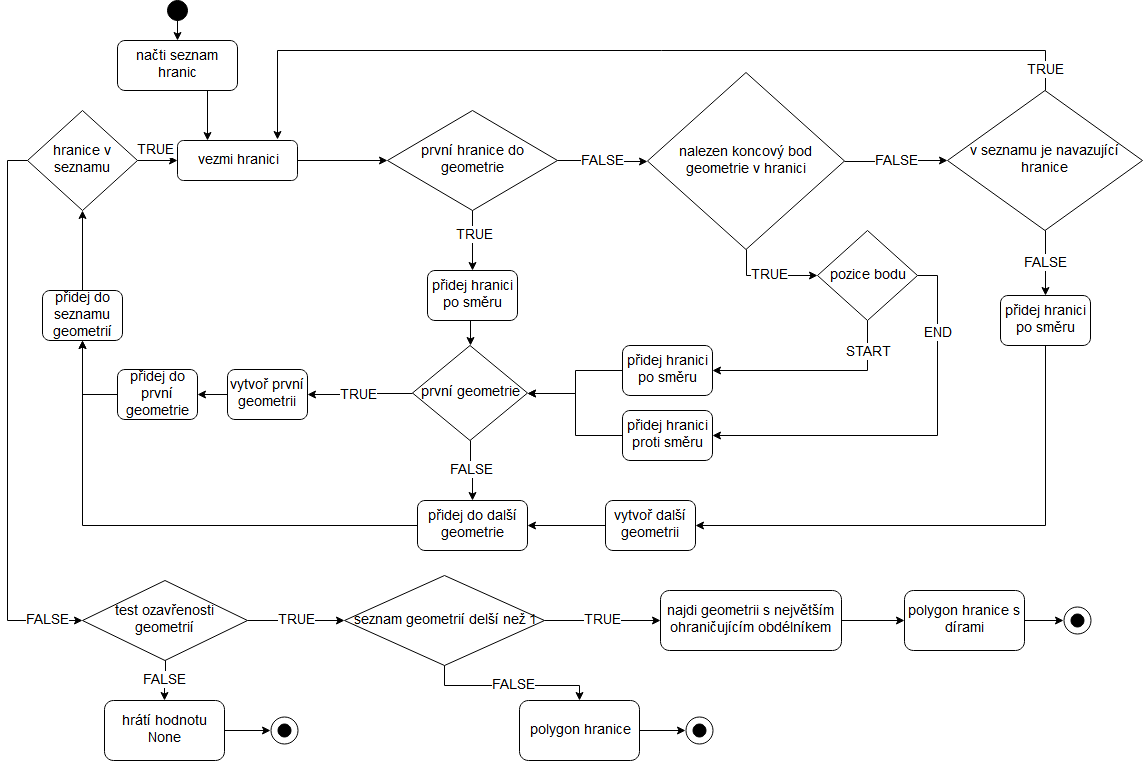
\includegraphics[width=15cm]{./pictures/Diagram_sestaveni_geometrie_hranic.png}
      \caption{zdroj:vlastní}
      \label{fig:logika_geometrie}
  \end{figure}
  
 \section{Ukázka načtení dat pomocí zásuvného modulu v prostředí QGIS}
 \label{sec:nacteni_dat_ukazka}
 \begin{enumerate}\bfseries
 \item{Spuštění zásuvného modulu kliknutím na ikonu \texttt{Otevřít prohlížeč VFK}}
  \begin{figure}[H]
	 \centering
      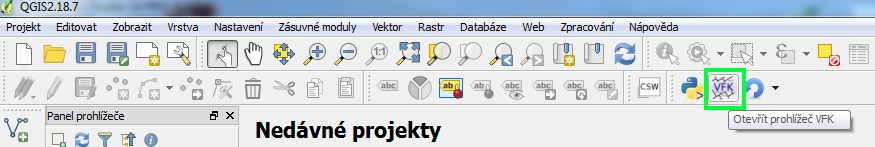
\includegraphics[width=15cm]{./pictures/nacteni_1kr.png}
      \caption{Ikona zásuvného modulu (označena zeleně)}
      \label{fig:1kr_nacteni}
  \end{figure}
  
  \newpage
  \item{Pro výběr VFK souboru stiskněte tlačítko \texttt{Procházet} (označeno zeleně)}
  \begin{figure}[H]
	 \centering
      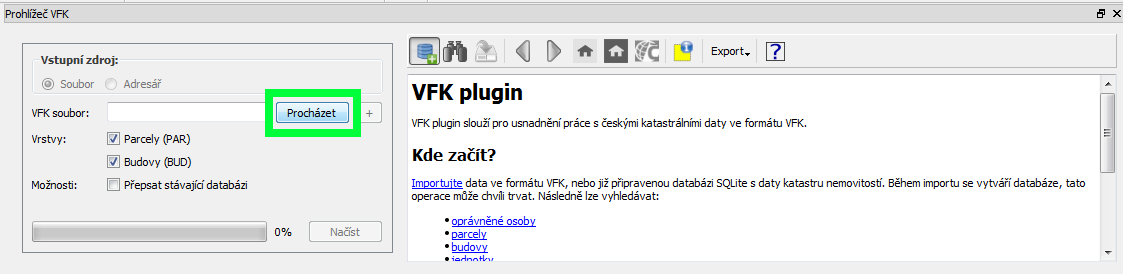
\includegraphics[width=15cm]{./pictures/nacteni_2kr.png}
      \caption{Výběr VFK souboru}
      \label{fig:2kr_nacteni}
  \end{figure}
  
  \item{Zvolení VFK souboru a výběr kliknutím na tlačítko \texttt{Otevřít}, výběr možný i dvojklikem}
  \begin{figure}[H]
	 \centering
      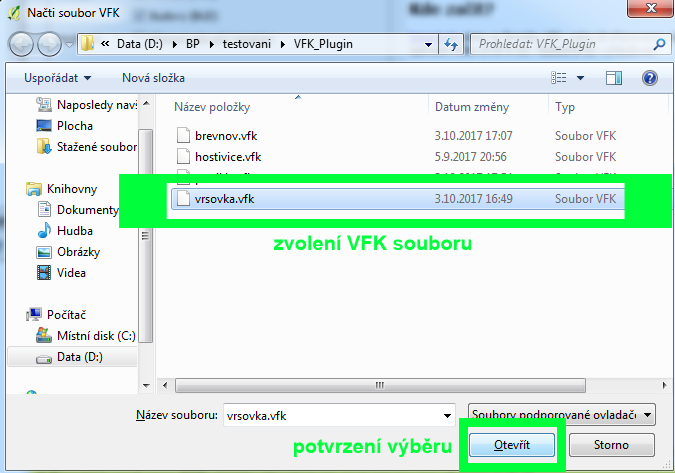
\includegraphics[width=15cm]{./pictures/nacteni_3kr.png}
      \caption{Načti soubor VFK}
      \label{fig:3kr_nacteni}
  \end{figure}
  
  \newpage  
  \item{Kliknutím na tlačítko \texttt{Načíst} se spustí načítání dat}
  \begin{figure}[H]
	 \centering
      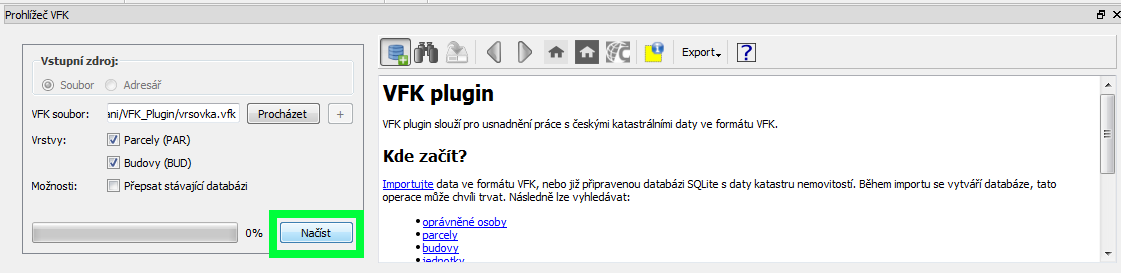
\includegraphics[width=15cm]{./pictures/nacteni_4kr.png}
      \caption{Spuštění načítání}
      \label{fig:4kr_nacteni}
  \end{figure}
  
  \item{Probíhá načítání}
  \begin{figure}[H]
	 \centering
      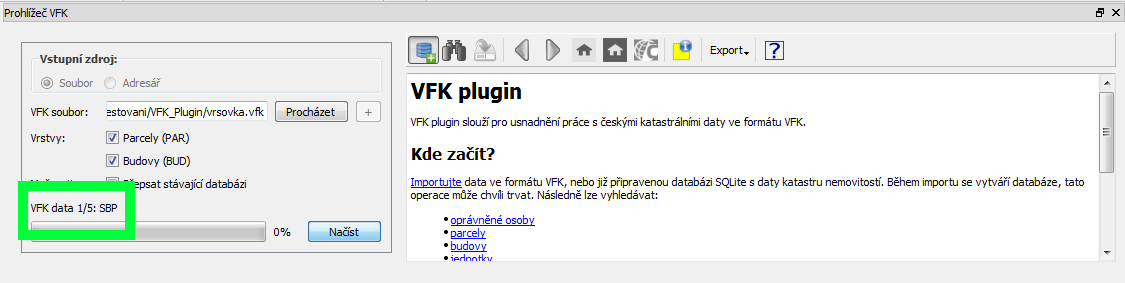
\includegraphics[width=15cm]{./pictures/nacteni_5kr.png}
      \caption{Načítání v procesu, může chvíli trvat}
      \label{fig:5kr_nacteni}
  \end{figure}
  
   \item{Data se po načtení sama zobrazí}
  \begin{figure}[H]
	 \centering
      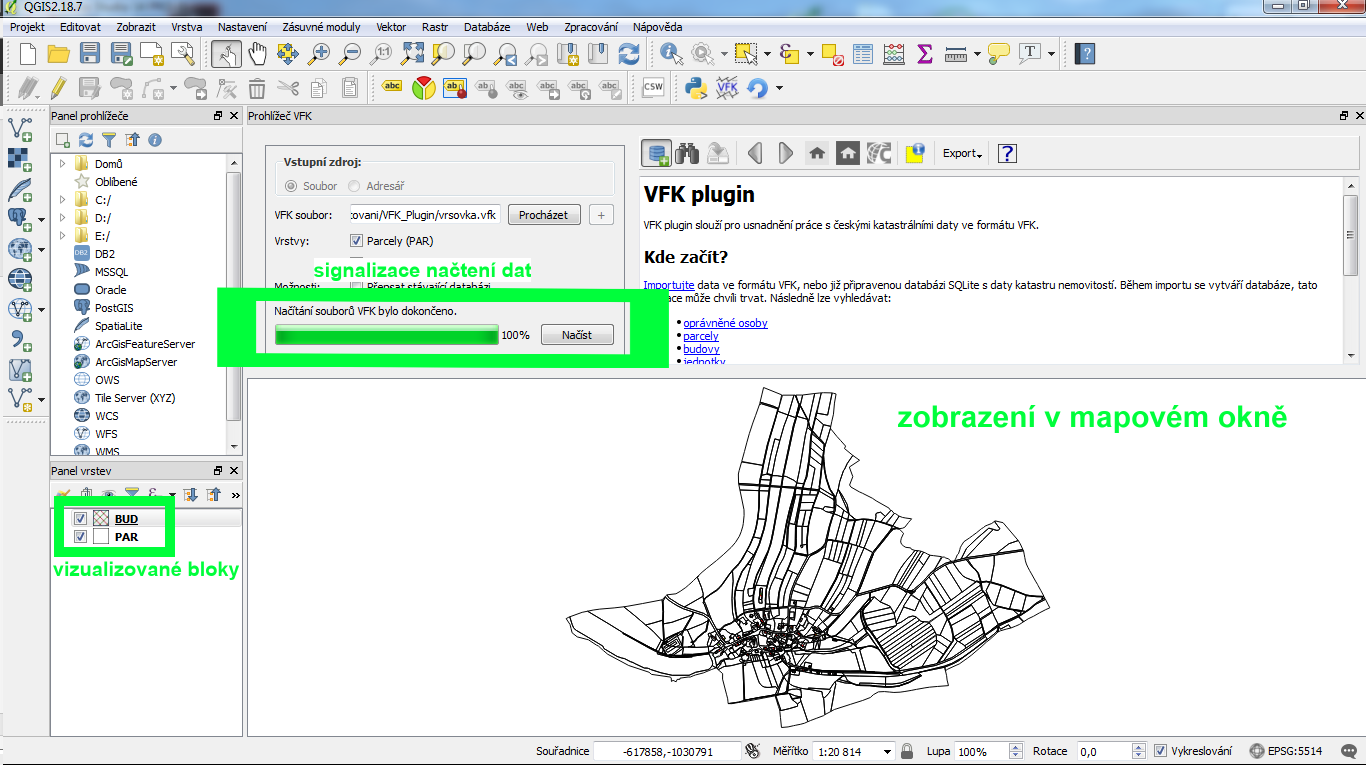
\includegraphics[width=15cm]{./pictures/nacteni_6kr.png}
      \caption{Načtená data pro obec Vršovka}
      \label{fig:6kr_nacteni}
  \end{figure}
 \end{enumerate}
 
 \section{Ukázka stažení veřejně poskytovaných dat VFK}
 \label{sec:stazeni_dat_ukazka}
  \begin{enumerate}\bfseries
  \item{Katastrální mapa poskytovaná v různých formátech}
  \begin{figure}[H]
	 \centering
      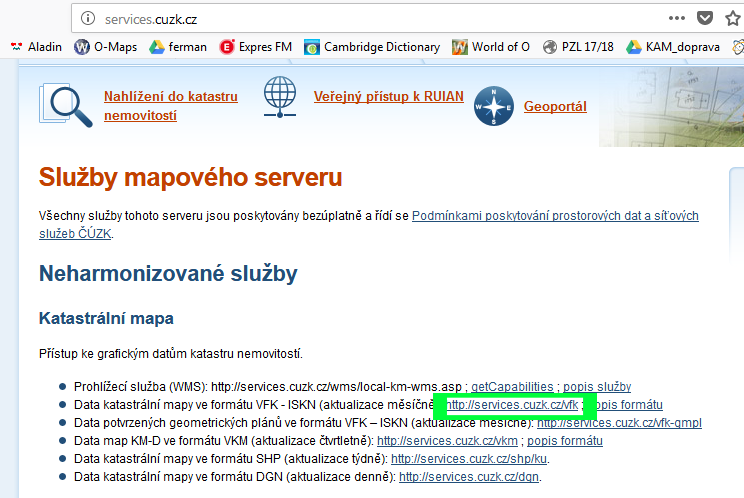
\includegraphics[width=15cm]{./pictures/stazeni_dat_1kr.png}
      \caption{Výběr dat ve formátu VFK (označeno zeleně)}
      \label{fig:1kr_stazeni}
  \end{figure}
  
  \item{Volba parametru vymezujícího oblast dat}
  \begin{figure}[H]
	 \centering
      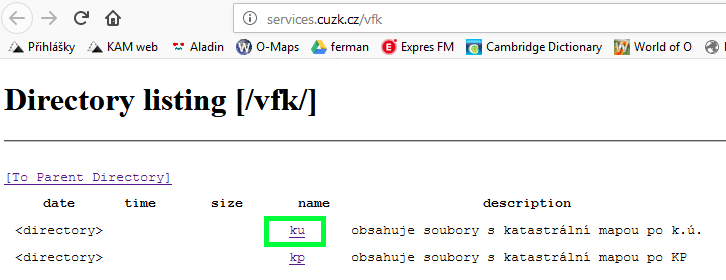
\includegraphics[width=15cm]{./pictures/stazeni_dat_2kr.png}
      \caption{Výběr dle katastrálních území(ku) (označeno zeleně)}
      \label{fig:2kr_stazeni}
  \end{figure}
  
  \newpage
  \item{Volba dne vytvoření dat}
  \begin{figure}[H]
	 \centering
      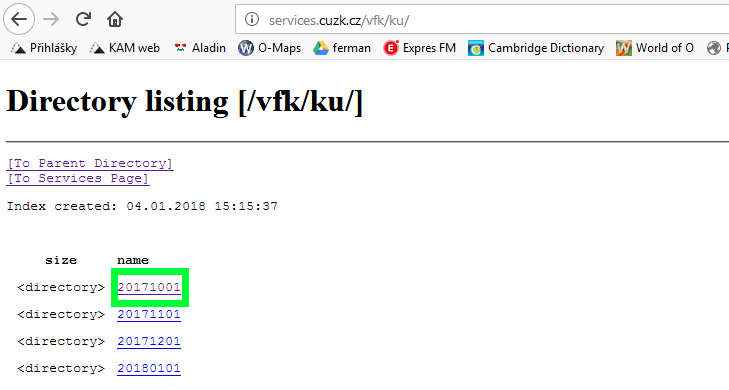
\includegraphics[width=15cm]{./pictures/stazeni_dat_3kr.png}
      \caption{Výběr 1.10.2017 (označeno zeleně)}
      \label{fig:3kr_stazeni}
  \end{figure}
  
  \item{Volba konkrétního katastrálního území, řazeno abecedně}
  \begin{figure}[H]
	 \centering
      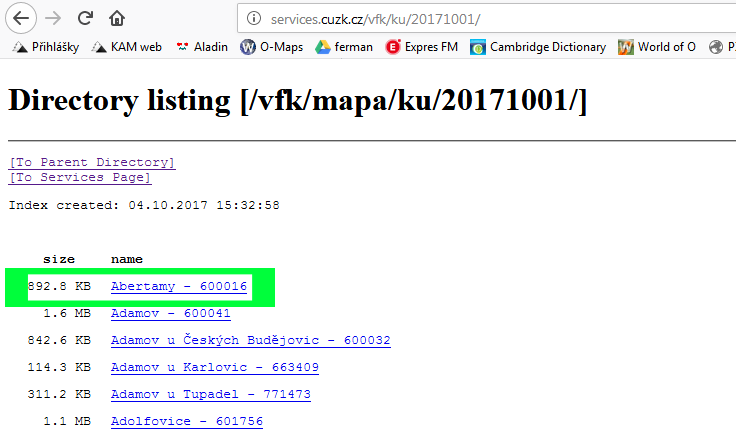
\includegraphics[width=15cm]{./pictures/stazeni_dat_4kr.png}
      \caption{Výběr Abertamy - 600016 (označeno zeleně)}
      \label{fig:4kr_stazeni}
  \end{figure}
  
  \newpage
  \item{Stažení a uložení zvolených dat}
  \begin{figure}[H]
	 \centering
      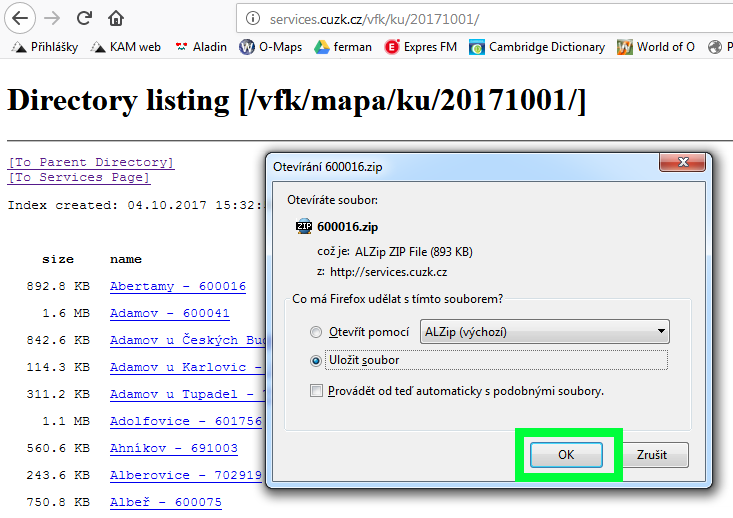
\includegraphics[width=15cm]{./pictures/stazeni_dat_5kr.png}
      \caption{Potvrzení výběru tlačítkem OK (označeno zeleně)}
      \label{fig:5kr_stazeni}
  \end{figure}
  \end{enumerate}

\chapter{Obsah přiloženého CD}
\label{cd}
 %% ML: zde bude v podstate obsah gitu + pdf
 %% LK: diff bude ve slozce src?

\setlength{\unitlength}{.5mm}
\begin{picture}(250, 220)

  \put(  0, 212){\textbf{.}}

  \put(  1, 200){\line(0, 1){5}}
  \put(  1, 200){\line(1, 0){10} {\textbf{ src}}} 
  \put(150, 200){ zdrojový kód}  

  \put(  1,  190){\line(0, 1){10}}
  \put(  1,  190){\line(1, 0){10} {\textbf{ sample\_data}}}
  \put(150,  190){ testovací data}                     
          
  \put(  1,  180){\line(0, 1){10}}
  \put(  1,  180){\line(1, 0){10} {\textbf{ text}}}
  \put(150,  180){ text práce ve formátu PDF}
      
  \put(  1,  170){\line(0, 1){10}}
  \put(  1,  170){\line(1, 0){10} {\textbf{ zadani}}}
  \put(150,  170){ zadání bakalářské práce}
\end{picture}

% Konec dokumentu
\end{document}
